\chapter{Model parametrisation}\label{ch:parametrisation}

Before applying the model to solve fishery management problems we need to be confident of the reliability of model predictions; hence, we first need to work on achieving the model dynamics under tight coupling of model predictions to observations. In the fields of numerical modelling of physical phenomena in atmosphere and ocean, this is referred to as ``data assimilation'', and in ecology it is called quantitative modelling; the purpose of both is the same -- to provide the estimates of nature, which are better estimates than can be obtained by using only the observational data or only the dynamical model (Robinson and Lermusiaux, 2002). Hence, quantitative modelling relies on integrating as much available data as is necessary to observe (and constrain) model dynamic processes through all considered dimensions. In fish population dynamics modelling, we do not directly observe the model variables, that is, fish biomass, so we cannot use inverse methods to correct the model state as is done in meteorological or ocean circulation models. Instead, we use inverse methods to compute the gradient of the function of model parameters and observations with the aim to inform model parameters from the data, which contains observations for different processes of fish population dynamics. As an outcome, we want to achieve an optimal model parametrisation providing the model (i) describes the assimilated data and (ii) remains valid for independent data sets. The latter can be fulfilled through space--time invariance of model parameters. Indeed, the SEAPODYM parameters, proper to the modelled species and its physiological characteristics, do not include dependencies on its environment. In contrast, they describe the species response to the environment that is included in the model as the forcing data. This chapter describes methods implemented in SEAPODYM to assist in the development of quantitative models. These methods, however, should not be considered as ready-to-use or universal recipes for building quantitative models for the new species with SEAPODYM as this process involves solving highly dimensional non-linear optimization problems and the success depends strongly on the amount of observations available. 

\section{Integrating data in a fish population dynamics model}\label{sec:integrating-data}

Since SEAPODYM is a spatio-temporal model with age dynamics, describing the entire population life cycle, it possesses high dimensionality that inevitably requires the use of massive geo-referenced datasets. For tuna species we use three types of geo-referenced data: (1) fisheries data, including effort and catch aggregated in time and spatial area; (2) length frequency sample data provided at usually coarser resolutions, such as season and large regions; and (3) conventional tagging data including the positions of release and recapture as well as size characteristics of individual fish. It is important to note here that fisheries data must account for as close to 100\% of fishing mortality as possible (Figure~\ref{fig:annual_catches}) to enable unbiased estimation of population abundance, but it is not required that all fisheries data are used in the parameter estimation method. 
 
\begin{figure}[H]
\begin{center}
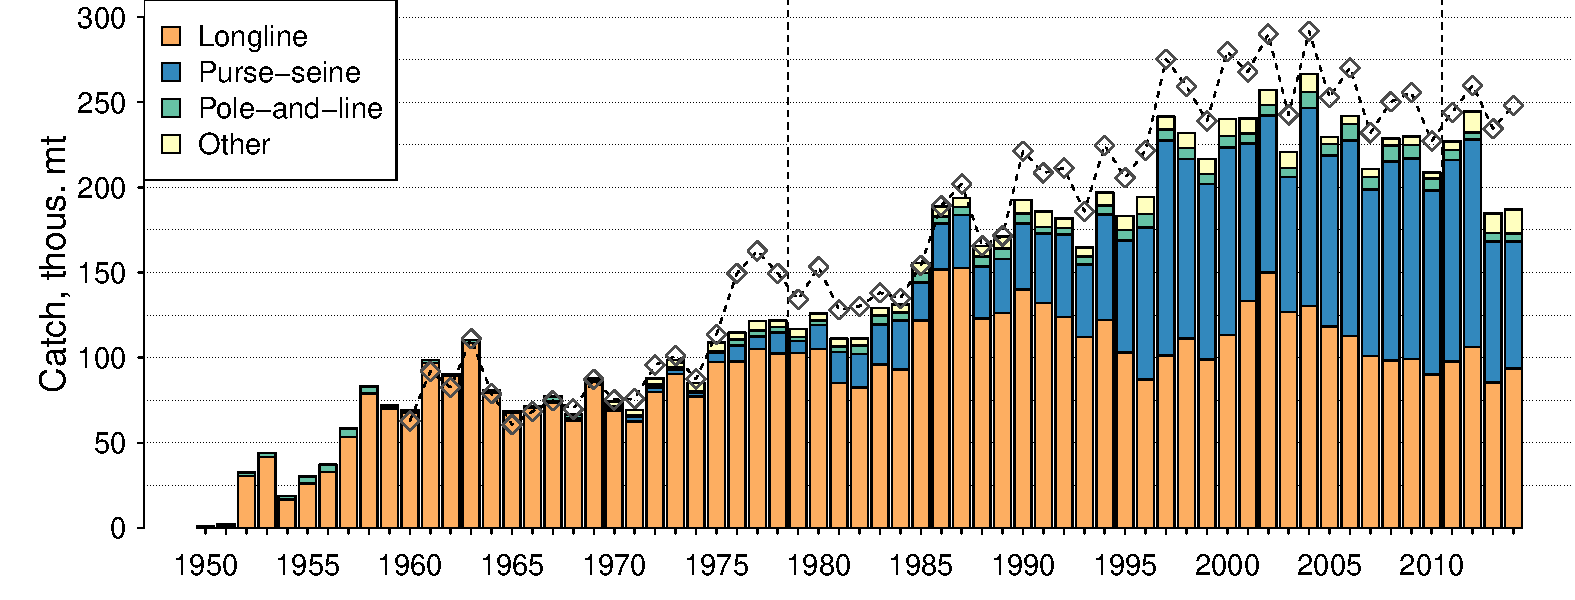
\includegraphics[width=1.0\textwidth]{chapter4/figs/bet_catch_bars}
\caption{Total annual bigeye tuna catch aggregated from geo-referenced catch (Pacific-wide) used in SEAPODYM analyses. The dashed line corresponds to total landings of bigeye tuna \citep{Yearbook}. }
\label{fig:annual_catches}
\end{center}
\end{figure}

\subsection{Effort and catch data}\label{sec:integrating-catch}

Geo-referenced fishing data include effort and catch by flag, gear and fishing strategy. These data on tuna and billfish are collected by Tuna Commissions and are publicly available to a certain level of detail. The following Tuna Commissions contributed to the SEAPODYM studies: the Inter-American Tropical Tuna Commission (IATTC) for  the eastern Pacific Ocean, the Pacific Community (SPC) on behalf of the Western Central Pacific Fisheries Commission (WCPFC) for the western and central Pacific Ocean, the Indian Ocean Tuna Commission (IOTC) for the Indian Ocean and International Commission for the Conservation of Atlantic Tunas (ICCAT) for Atlantic Ocean. The large industrial fishing fleets targeting different tuna species use several gears -- purse-seine (PS), pole-and-line (PL), longline (LL) and troll (T). Typically, for tuna species, monthly spatially distributed data on large-scale industrial and small-scale domestic fishing are available for effort, $E_{t,f,lon,lat}$, as a number of sets, days fishing or a number of hooks; and catch, $C^{obs}_{t,f,lon,lat}$, in weight or number of fish (see Fig.~\ref{fig:catches_maps}), where indices $t,f,lon,lat$ refer to the year-month, fleet, and geographic coordinates of 1-degree cells.

\captionsetup[subfigure] {labelformat=empty,labelfont=bf,textfont=normalfont,singlelinecheck=on}
\begin{figure}[H]
\centering
\begin{subfigure}[b]{0.485\textwidth}
\caption{1980s}
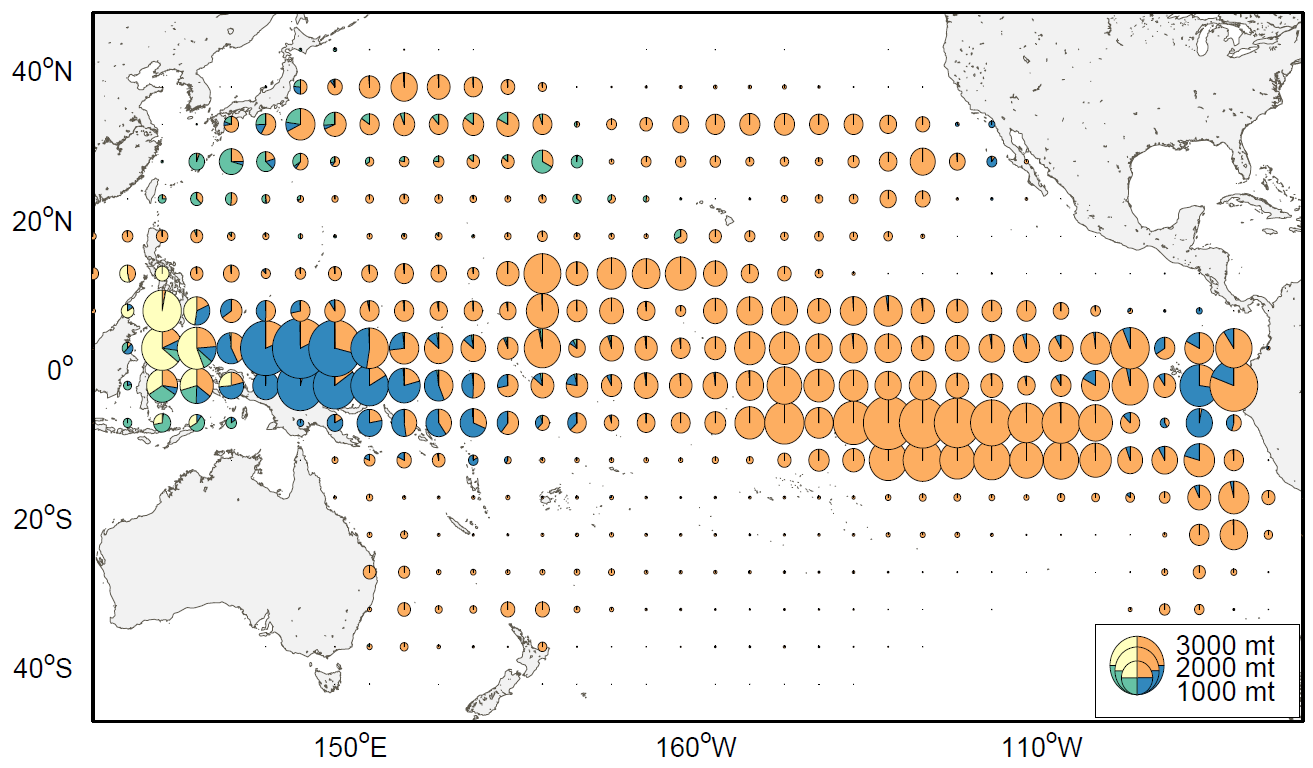
\includegraphics[width=1\textwidth]{chapter4/figs/bet_catch_2d_80s}
\end{subfigure}
\begin{subfigure}[b]{0.485\textwidth}
\caption{1990s}
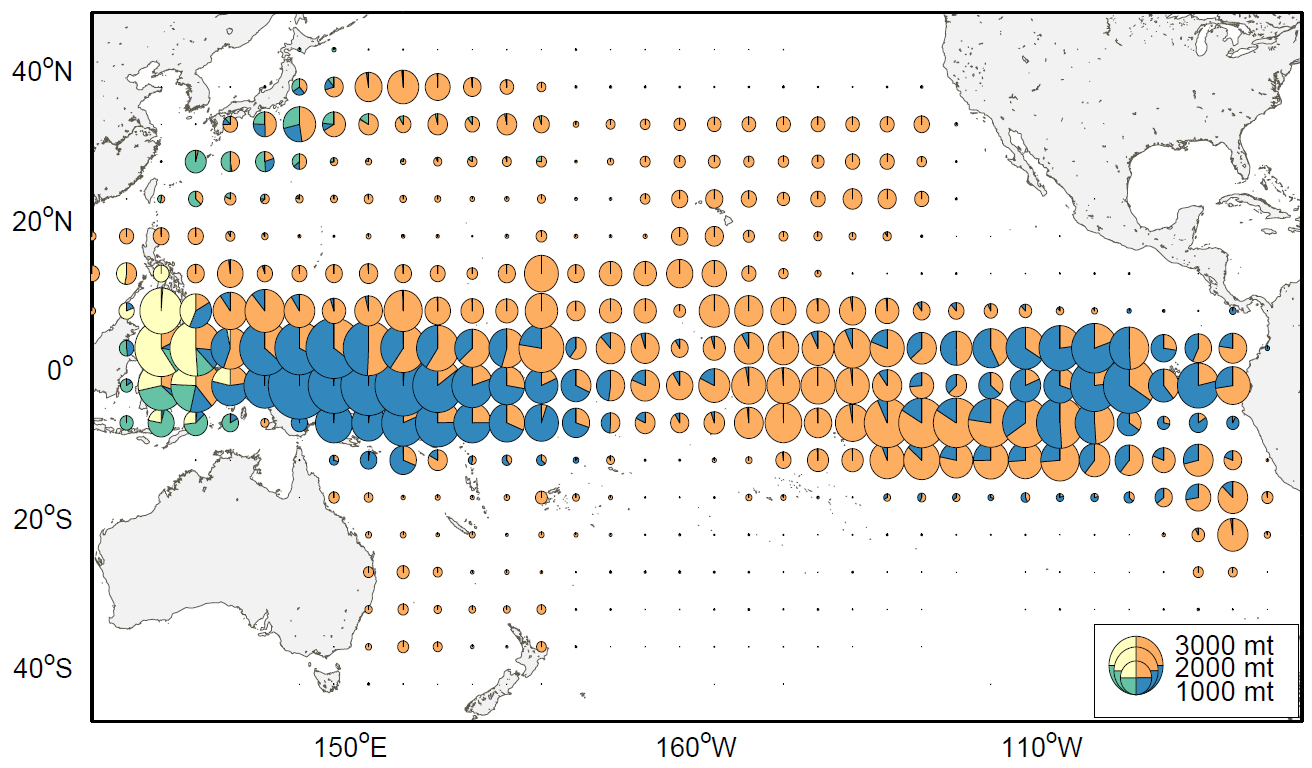
\includegraphics[width=1\textwidth]{chapter4/figs/bet_catch_2d_90s}
\end{subfigure}
\begin{subfigure}[b]{0.485\textwidth}
\caption{2000s}
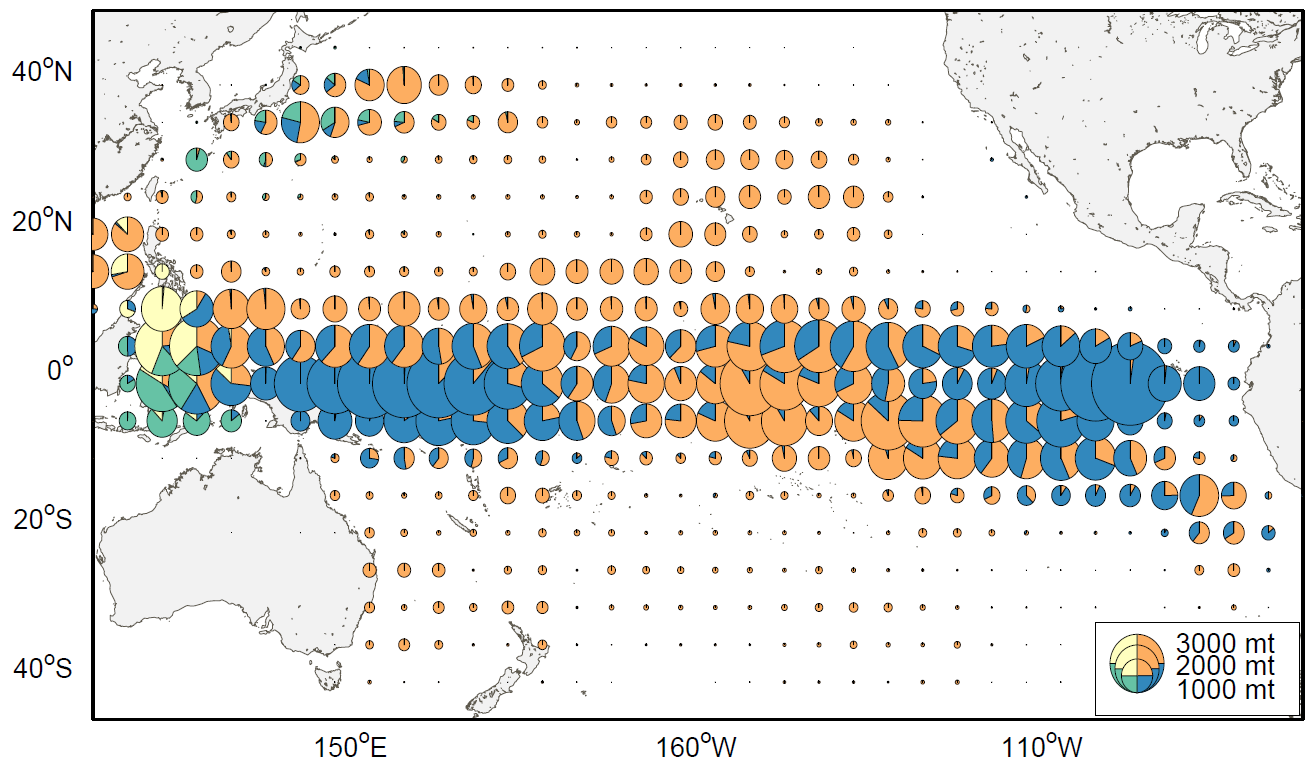
\includegraphics[width=1\textwidth]{chapter4/figs/bet_catch_2d_00s}
\end{subfigure}
\begin{subfigure}[b]{0.485\textwidth}
\caption{2010s}
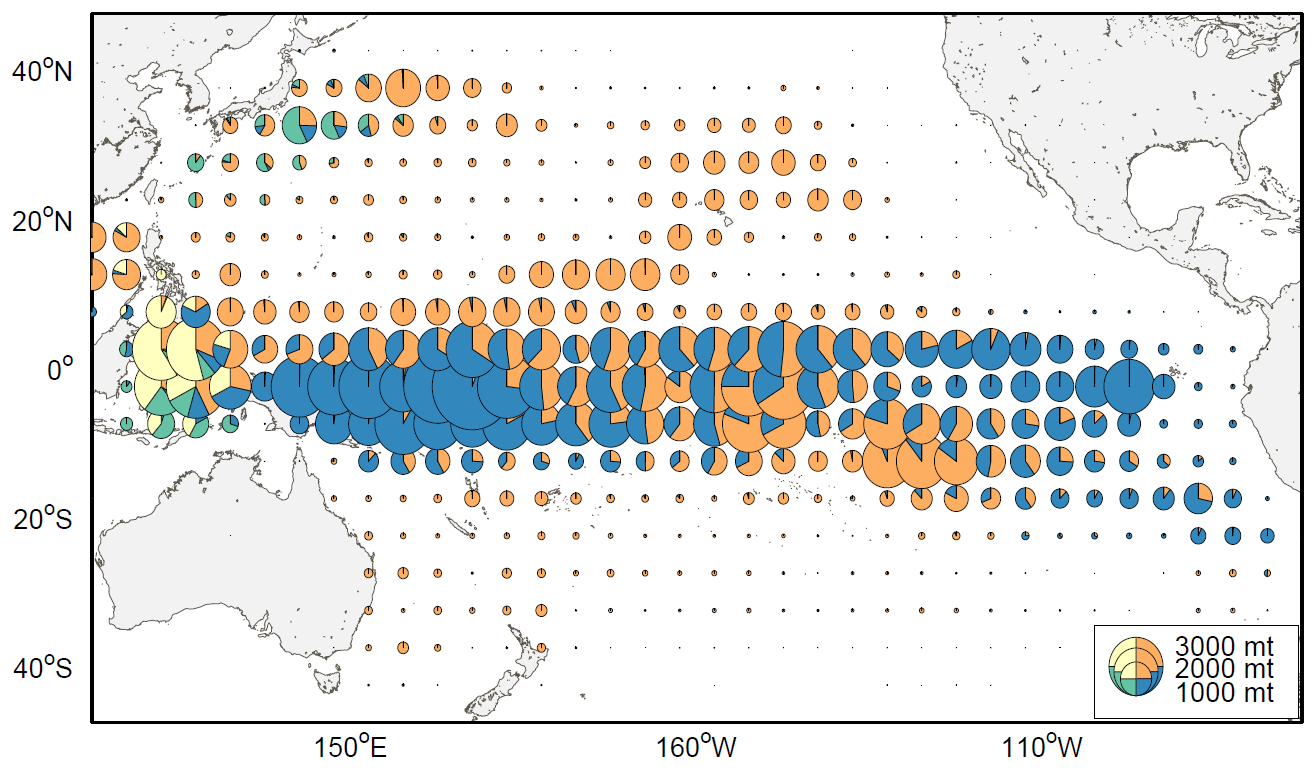
\includegraphics[width=1\textwidth]{chapter4/figs/bet_catch_2d_10s}
\end{subfigure}
\caption{Spatial distributions of bigeye tuna catches by decade and by gear: longline (orange), purse-seine (blue), pole-and-line (green), and others (yellow).}
\label{fig:catches_maps}
%\end{center}
\end{figure}

Prior to integrating these data into SEAPODYM for parameter estimation, it is important to organise them into homogeneous fisheries. The latter are defined in SEAPODYM by a unique selectivity function, which does not depend on space and time, and by a unique catchability coefficient, which can only change linearly with time. The linear trend may be necessary to account for technological advances, affecting the time of searching and volumes of fish being caught. Spatial and temporal variability in catch is assumed to be driven by the spatial distributions of fish that are explicitly described by the model. Another source of variable catchability,  oceanographic features such as fronts and eddies, are accounted for as well through the habitat and movement modelling. The habitat index reflects both thermal gradients and the concentrations of prey species, transported and organised into heterogeneous spatial structures by ocean currents. Hence, the gradual changes in fisheries, such as geographic expansion or seasonal displacements of fishing grounds, and the continuous increase in fishing effort and catch (Figure~\ref{fig:catches_maps}) can be successfully integrated. In contrast, all abrupt changes in fisheries parameters due to changes in fishing strategy and target species, introduction of regulatory measures, whether seasonal or not, need to be eliminated by splitting the fleet data. Usually, this information can be derived either from Commissions' reports, from the provided fisheries descriptions, or by conducting the time series analysis. Finally, the data with unreliable, partially available fishing effort should also be removed from fisheries whose data will be integrated within the parameter estimation method. Such fisheries can be accounted for with the help of the catch removal method described below. 

\subsubsection{Catch prediction methods} \label{sec:predicted-catch}

Previous studies with SEAPODYM using fisheries data to inform model parameters indicated several problems with the use of fishing effort, in particular those for purse-seine gear. Using fishing effort to predict the catch in each observed spatial position logically results in fish distributions with the centre of mass shifted to the areas with highest CPUE and the lowest biomass in areas with the lowest CPUE. The highest CPUE can be due to highest biomass, but also to lowest effort and in purse-seine data, where the fishing effort, expressed in days, may include time unrelated to fishing, it is often observed that the CPUE is lowest in the main fishing grounds, and highest on the edges of the fishing grounds. Fitting the model predictions by relying on such effort leads to biases and excessive dispersal and hence overestimation of fish density away from the observed locations, creating a large quantity of non-observed ``cryptic'' biomass, which might be unrealistic. The term ``cryptic'' biomass was first introduced by \citet{Fonteneau} for the fraction of the stock that is unavailable to fisheries. To avoid such biases, there are two catch prediction methods in SEAPODYM: the classical Gordon-Schaefer formula and the catch removal method (see also the fishing mortality section~\ref{sec:FM}). 

The first method is based on the fishing effort. The total mortality of all fish of age $a$ due to fishing, $m_F(a)$, eq.~\ref{eq:FM}, depends on the catchability coefficients, $q_f$, of fisheries $f$, their selectivity, $s_{fa}$, for the fish at age $a$, and the observed fishing effort, $E_{f}$. At every spatial location and time, the instantaneous total catch $C$ in number of fish of age $a$ is computed as follows: 

\begin{align}
&C(a) = m_F(a) \cdot N(a) \cdot A_{xy}, 
\label{eq:GS-catch-prediction}
\end{align}

\noindent where $N(a)$ is modelled density of fish in number of individuals per unit area (Nb/km$^2$), and $A_{xy}$ is the area in km$^2$. However, observations are available for the large time intervals and spatial area. Passing to numerical model notations (see sections~\ref{sec:d-space}--\ref{sec:d-age}), we define $C^{\text{pred}}_{fKIJ}$, the total predicted catch in mass units (mt -- metric tonnes) by fishery $f$ at outer time step $K$ and observational grid indices $(I,J)$ as:

\begin{align}
C^{pred}_{fKIJ}=q_f E_{fKIJ} \sum\limits^{n_a}_{p=0} s_{fp} w_p \sum\limits_{ij \in IJ} N_{pKij} {\scriptstyle\Delta} x_i \mathit{\scriptstyle\Delta} y_j,
\label{eq:catch-in-weight}
\end{align}

\noindent where $w_p$ is the mean weight of fish and $N_{pKij}$ is the density of fish in the $p$-th age class and numerical grid indices $(i,j)$. As seen in this formula, the effort data should be provided at the model's temporal resolution; however, the spatial resolution of observations can be retained. It allows the effort to be applied to the model biomass after its aggregation to the larger area, and the predicted catch to be compared to observed catch at its original resolution. Note that the prediction of catch rate, that is, catch per unit of effort by fishery, is straightforward with this catch prediction method. The prediction of catch per unit of effort at the resolution of observations, $\text{CPUE}^{pred}_{fKIJ}$, is obtained by division of  eq.~\ref{eq:catch-in-weight} by the effort value, $E_{fKIJ}$. 

Thus, the predicted catch depends not only on the available fish biomass, but also on the fishing effort, gear catchability and selectivity. Since the selectivity parameters do not vary in space and time (with catchability either constant or allowed to change linearly over time), the estimation of population spatial distribution in the MLE approach is essentially driven by the spatio-temporal variations of the biomass and the fishing effort. Unfortunately, this approach is correct only in the ideal case, that is, when the fishing effort is well estimated and fully reported. For gears such as purse-seine, the estimation of fishing effort is problematic as one should take into account not only the number of sets that were employed after the fish school had been detected, but also the time the boat spent in active searching. The second variable is often hard to estimate and usually the effort becomes inflated in the principal fishing grounds characterised as zones with the highest catches and where the fishing boats spend more time and is underestimated in the areas, which are rarely visited by the fishers. As an example, the observed CPUE of purse-seine fisheries targeting free schools of skipjack tuna are higher outside the main fishing grounds, thus showing a clear density gradient towards their edges. One can also imagine that using equation \ref{eq:GS-catch-prediction} in MLE in the case when the catch is highly correlated with the effort will lead to estimating a homogeneous distribution of biomass. Another problem can arise with the effort of those fisheries that do not target the modelled species or change the target during their fishing campaign. If the information about currently targeted species is not contained in the fishing effort, the biomass estimation becomes biased because zero catch does not necessary reflect the absence of the non-target species.

To avoid the biases associated with the use of inaccurate fishing effort, another method was implemented in SEAPODYM. It consists of removal of total (summarised over all fisheries) catch in number of fish of a given age class directly from the predicted fish density. Let us denote $N_{pkij}$ as the population density in number of fish of age class $p$ per unit area at the model integration step $k\frac{\Delta T}{n}$ ($k=1\dots n$, $n$ -- number of iterations in the ADI method); $C^{\text{obs}}_{pkij}=\frac{1}{n}C^{\text{obs}}_{pKij}$ is the \textit{n}th portion of the total observed catch at time interval $(T_K, T_{K+1})$. Then the corresponding predicted catch at the ADI method sub-step is computed as follows:

\begin{align}
&C^{\text{pred}}_{pkij} = \text{min}\left(C_{pkij}^{\text{obs}}, (N_{pkij} \cdot \scriptstyle{\Delta} x_i \scriptstyle{\Delta} y) \right).
\label{eq:CR}
\end{align}

Note, that according to eq.~\ref{eq:CR} the predicted catch is either equal to or less than the observed one. The latter occurs only if there is not enough biomass in the model grid cell. Finally, the predicted total catch is summed up through $n$ ADI iterations and the total value is attributed to the fisheries $f$ operating in the cell $ij$ according to their observed ratio in this cell, that is,

\begin{align*}
C^{\text{pred}}_{fpKij} = \frac{C^{\text{obs}}_{fpKij}}{\sum_f C^{\text{obs}}_{fpKij}} \sum_{k=1}^n C^{\text{pred}}_{pkij},
\label{eq:CR-catch-at-age}
\end{align*} 

\noindent gives the catch by fishery at model temporal and spatial resolutions. So, in contrast to the first method, this approach requires data redistribution, which is done automatically in the model software.

Equations~\ref{eq:CR} and \ref{eq:MCR} can be combined with the classical eqs.~\ref{eq:catch-in-weight} and \ref{eq:FM} by applying the Gordon-Schaefer formula to selected fisheries, for which the fishing effort can be considered unbiased (longline and pole-and-line fisheries targeting modelled species). One inconvenience of the catch removal approach is that it cannot combine catch data with different units (e.g., metric tonnes and numbers of fish).  

\subsection{Length frequency data}\label{sec:integrating-lf}

The length frequency (LF) data are the geo-referenced sample data, including information on flag, gear, fishing method, temporal interval, region and sampled catch at length (raised or not), and the total catch by a given fleet. However, these data are usually aggregated by quarter and over larger areas, for example, $5^{\circ} \times 5^{\circ}$, $5^{\circ} \times 10^{\circ}$, $10^{\circ} \times 10^{\circ}$ or larger (see Figure~\ref{fig:lf-data}). Note, the fisheries structure in LF data must be conformal to that in the effort and catch dataset. 

\subsubsection{Length frequency prediction}

By definition, the length frequency is the proportion of fish of size $\ell(a)$ observed in the catch by fishery $f$ at time $t$ and in region $r$. Since SEAPODYM is an age-structured model, we need to redistribute the catch-at-length to catch at the mean length of model age classes, which is in most cases straightforward as the model age classes usually have a coarser resolution than the observed length bins. In discrete space and time notation, the predicted LF, denoted $Q^{\text{pred}}$, is computed as follows:

\begin{equation}
 Q^{\text{pred}}_{fpKr}=\frac{s_{fp} \sum\limits_{i,j \in r} E_{fij} N_{pKij}{\scriptstyle\Delta x_i} {\scriptstyle\Delta y_j}}{\sum\limits^{n_a}_{p=0} s_{fp} \sum\limits_{i,j \in r} E_{fij} N_{pKij}{\scriptstyle\Delta x_i} {\scriptstyle\Delta} y_j}
\label{eq:LF}
\end{equation}

\noindent where selectivities $s_{fp}$ are described in eq.~\eqref{eq:fishery-specific-selectivity}, $ij \in r$ are the indices of the model grid, region $r$ is defined by observations, $\Delta x_i$ and $\Delta y_j$ are grid cell sizes as defined in section~\ref{sec:d-space}. 

\begin{figure}[htbp]
  \centering
  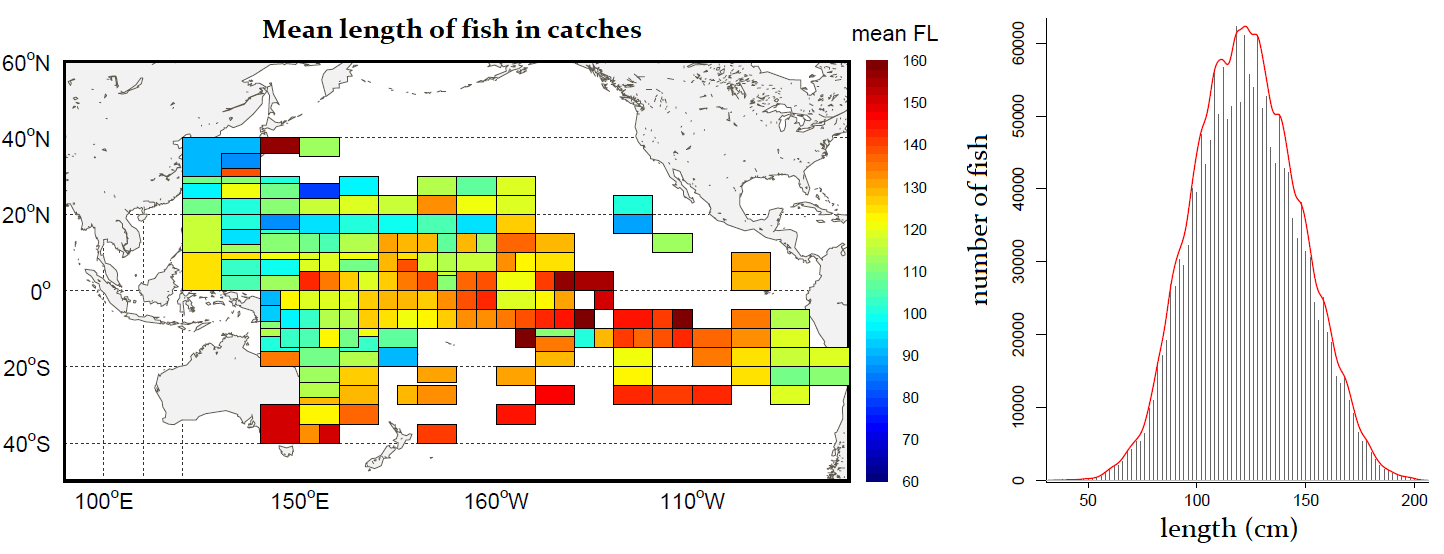
\includegraphics[width=1.0\textwidth]{chapter4/figs/LF-data}\\
  \caption{Typical length frequency dataset comprising distributions of fish sizes in catch withdrawn in multiple sample regions. The colour on the left-hand side of the map indicates the mean fork length (FL) of fish caught in each region. The vertical lines on the histogram show the sampled number of fish at a given size. The solid red line corresponds to the kernel density estimation for the data sample.}
  \label{fig:lf-data}
\end{figure}

\subsection{Conventional tagging data}\label{sec:integrating-tags}

Conventional release--recapture tagging data include information on position, date and size of the fish upon release and the same information upon fish recapture (Figures~\ref{fig:tag-data1} and \ref{fig:tag-data2}). Tagging campaigns are regularly conducted in the Pacific Ocean by SPC and IATTC under different tuna tagging programs, which started as early as 1967. In particular, SPC has conducted several large tagging experiments since the 1980s in the western and central Pacific Ocean (WCPO). For example, since 2008 SPC scientists deployed about 200,000 conventional tags on skipjack tuna. IATTC and the Japanese Fisheries Agency have been also very active in tuna tagging in the eastern and north-west Pacific respectively. While releases are made by fisheries scientists, the recaptures are by fishermen. Usually hundreds of tunas are released in a single location, and the spread of recapture locations depend on the fishing activity. Obviously, only a small proportion of the released fish is recaptured. The major difference between release and recapture data is its reliability. The data on releases are fully reported, while recordings of recapture locations and dates as well as the fish size upon recapture are subject to error. Therefore, special care is needed in preprocessing the tagging data, that is, verifying the boat positions through Vessel Monitoring System (VMS) data, and correcting or filling a gap on size information using known growth models for the species. 

\begin{figure}[H]
  \centering
  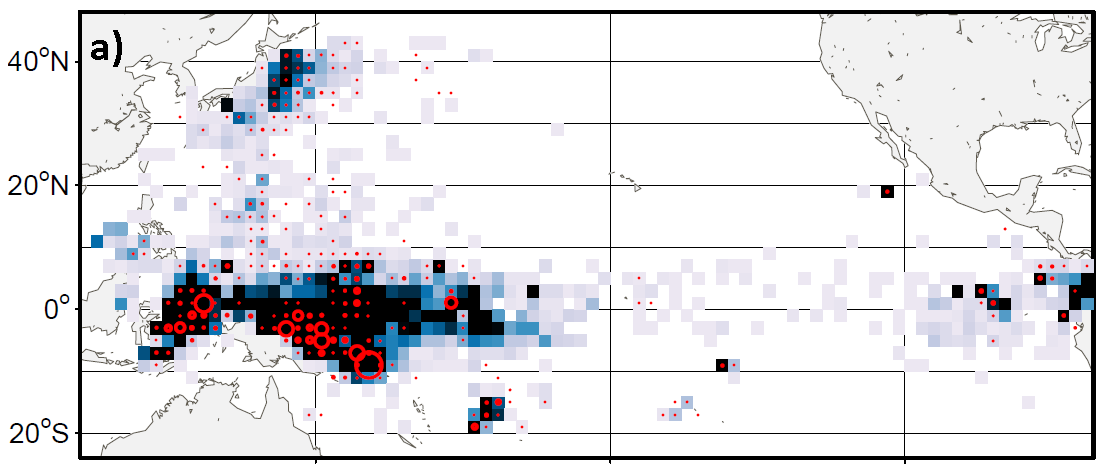
\includegraphics[width=0.75\textwidth]{chapter4/figs/tag-recaptures-skj}\\          
  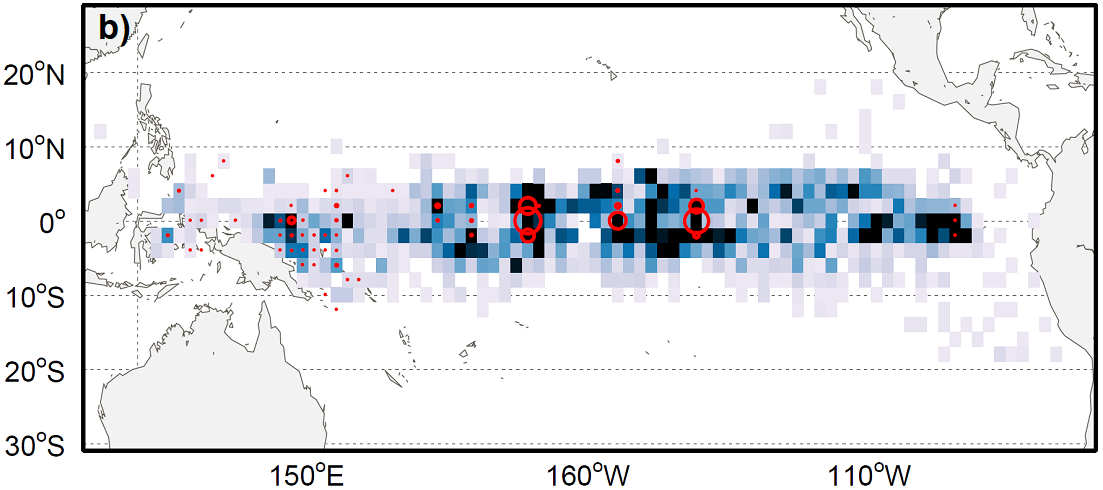
\includegraphics[width=0.75\textwidth]{chapter4/figs/tag-recaptures-bet}
  \caption{Number of skipjack (a) and bigeye (b) tunas that were tagged during conventional tagging campaigns (size of red circles is proportional to the number of released fish) and recaptured by industrial fishing vessels. The $1^{\circ}$ pixels are coloured with a linear colour scale from white to blue indicating 0 to 40 and more tag returns respectively.}
  \label{fig:tag-data1}
\end{figure}

There are other caveats in the use of conventional data. First, they do not allow observing of the entire population, but essentially the juveniles and immature adult fish that are associated with surface schools and can be caught with surface gears. For example, only juvenile and immature bigeye tunas were tagged and released along the equator (bottom panels in Figures~\ref{fig:tag-data1} and \ref{fig:tag-data2}). Second, a majority of all tagged tunas are recaptured shortly after release. For bigeye tunas, 89\% of all recaptured fish were recaptured within one year of liberty at sea, 10\% between one and two years and only 1\% after more than two years. Consequently, with size at 50\% maturity being 115 cm, the majority (93\%) of recaptures are still immature tunas. Hence, observing only part of the population may present difficulties for estimating model parameters responsible for the dynamics of an unobserved fraction of the population. Third, unknown reporting rates and strong dependence of tag recaptures on the associated geo-referenced fishing effort make it difficult to rely on these data in the estimation of natural mortality rates.

\begin{figure}[H]
  \centering
  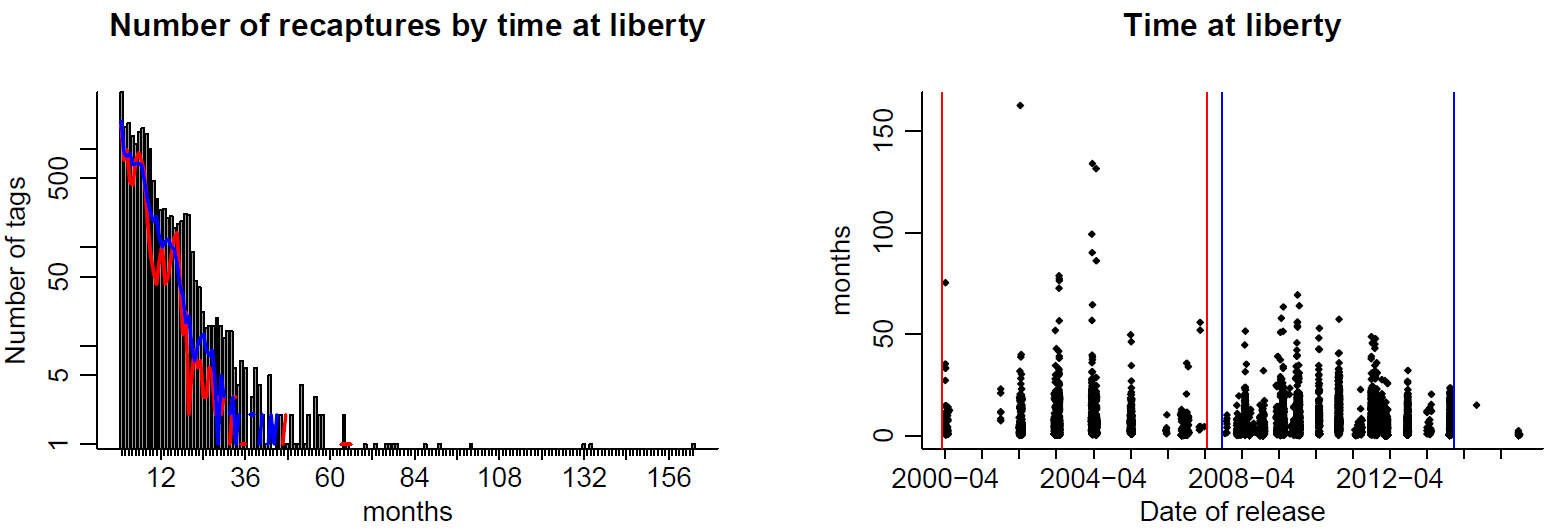
\includegraphics[width=0.85\textwidth]{chapter4/figs/tag-time-at-liberty}\\          
  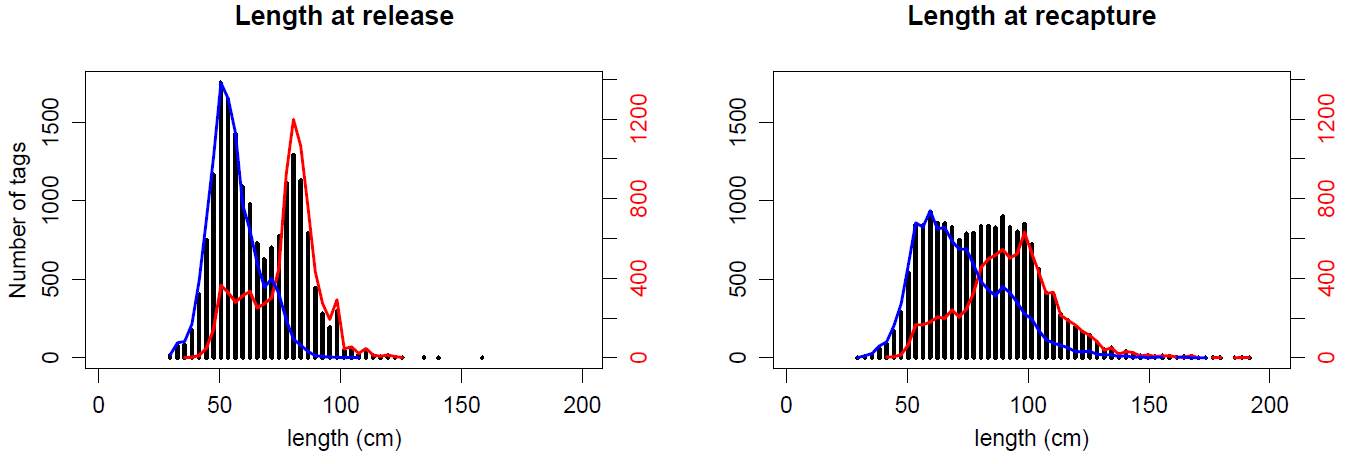
\includegraphics[width=0.85\textwidth]{chapter4/figs/tag-relrec-sizes}
  \caption{Available conventional tagging showing two distinct periods (enclosed by red and blue lines) in tagging data with different statistical properties of fish distribution. The histogram and scatter plot on time at liberty show the time at liberty frequency diagram and the time at liberty of the tags depending on their date of release, respectively. The size distributions at release and recapture depict the size (age) intervals that are observed by tagging data.}
  \label{fig:tag-data2}
\end{figure}

Conventional tagging data (Figure~\ref{fig:tag-data1}) are integrated into the optimization method in SEAPODYM essentially to improve the estimates of habitat and movement parameters that are critical to control the overall population dynamics. Therefore, the approach considers only fish that have been recaptured (see next section for more details), as these are the only data that contain information about potential movement \citep{Senina20b}. Nevertheless, compiled datasets of releases and recaptures, provided by SPC and IATTC from different tuna tagging programs, contain tens of thousands of records on released and consequently recaptured fish. 

For the purposes of reducing computational costs and integrating maximum information to inform dynamic processes through all model dimensions, it is important to choose the time period for data to be used by data assimilation methods. The criteria to be followed in making this choice are (1) the subset covers the time period without large gaps, (2) the subset does not reduce the observed time at liberty, and (3) the lifespan coverage of tagged fish is the same as for the whole dataset. For example, the tagging data temporal coverage and the distribution in terms of mean length and time at liberty illustrated in Figure~\ref{fig:tag-data2} reveal two characteristic periods with massive tagging of bigeye tuna within the 2000--2013 time range, clearly distinguished by the length of released tunas, the positions of release and the distributions of recaptures. During the first one, from early 2000 to mid-2007, the mean length of bigeye tuna at release was 77 cm; they were mostly tagged at three release positions around the equator at 95$^\circ$W longitude and a few dozen  tunas were tagged and recaptured in the warm pool area. During the second period, from mid-2007 to the end of 2013, much smaller bigeye tuna, 56 cm on average, were tagged, extending the area of release towards the central Pacific Ocean. So, providing a better coverage for spatial and age structure, the second subset of recaptures (2008--2013) constituting 50\% of the dataset (shown in Figure~\ref{fig:tag-data1}), panel (b) and in blue in Figure~\ref{fig:tag-data2}) is a better candidate for informing model parameters, while the first can be left for validation. 


\subsubsection{Movement model for tag prediction}\label{sec:model-tags}

The tagged fish represent a subset of the modelled population,and hence we can apply the same mathematical equations to describe their spatio-temporal dynamics. The approaches suggested earlier for Eulerian models \citep{Sibert} or used in the statistical stock assessment models \citep*[see e.g.,][]{Hampton-Fournier} rely on release--recapture data to inform estimations of both movement and natural mortality parameters. However, this approach is not practical within SEAPODYM. First, it leads to the augmentation of the model state vector by a large number of variables to describe the spatial dynamics of a tagged sub-population within the Eulerian model as we need to separate it into cohorts of fish being tagged and released at the same time and in the same area \citep{Sibert}. Second, tag reporting rates (the proportion of recaptured tags that are reported by fishermen) are not known. It means that a large proportion of tags might be recaptured and not reported, hence providing biased information on natural mortality. Calibrating the reporting rates within the parameter estimation is difficult because of their variation in space and time. Third, prediction of tag recaptures in this model depends on the quality of geo-referenced fishing effort and gear information. If these difficulties are not properly addressed, the information provided by tags on natural mortality may not ensure unbiased parameter estimation. At the same time, the main objective of integrating tagging data within SEAPODYM is to improve model predictions by adding information on fish movements. Hence, we must focus on modelling the movement of tagged fish. Since only recaptured tags can be informative of movement, we use only those released fish that were recaptured and reported. Because fish movements are essentially driven by the habitat indices based on environmental variables, the tagging data provide key information to estimate both habitat-related and movement parameters. 

Tags recaptured in the same month (quarter) are aggregated into cohorts. In other words, instead of defining the cohort by the same origin, it is defined by the same ending, that is, tags are aggregated into cohorts by their common time of recapture. As one cannot trace the density in an ADR model, this allows precise accounting for the time at liberty of all tags. Integration of tagging data within the population dynamic model (\ref{eq:model-1}-\ref{eq:model-3}) consists of adding the model of tag movement that is driven by the same model mechanisms and parameters. Let $R_k(a,t,\mathbf{x}), a=a_n,..,a_{n+\tau}$ be the density of the \textit{k}th cohort of tagged fish of age $a$, varying between the age at release $a_n$ and age at recapture $a_{n+\tau}$, where time at liberty,
$\tau$, is known from the recapture data. The variables $R_k$ are defined in two-dimensional space $\mathbf{x} \in \Omega \in \mathbf{R}^2$ and the time $t
\in (t_0,t_{R})$, where $t_0$ is the time of release of the first tag
in the cohort $k$ and $t_R$ is the time of recapture of all tags in
the cohort. The model of movement of the \textit{k}th cohort of tag density is based on a system
of advection--diffusion equations with ageing and source terms, zero initial and zero-flux boundary conditions:
\begin{linenomath}
\begin{align}{\label{eq:tagmodel}}
& \partial_t R_k+\partial_a R_k =-\text{div} (\mathbf v \cdot R_k ) +\nabla (D \nabla R_k) + r_k \\
& R_k(a,t_0,x)  = 0 \nonumber \\
& \mathbf n \cdot \mathbf v \Bigr\rvert_{\mathbf x \in \partial \Omega} = \mathbf n \cdot\nabla R_k \Bigr\rvert_{\mathbf x \in \partial \Omega} = 0 \nonumber
\end{align}
\end{linenomath}
where advection $\mathbf{v}$ and diffusion $D$ rates are the same as in the model~\ref{eq:model-1}, and the source term $r_k(a,t,\mathbf{x})$ includes all releases of age $a$ into cohort $k$ at time $t$. 

The model \hyperref[eq:tagmodel]{\ref*{eq:tagmodel}} with parameters of the model~\ref{eq:model-1}, included in the MLE approach, allows the estimation of movement and habitat parameters of model (\ref{eq:model-1}--\ref{eq:model-3}). Obviously, such an approach does not allow the estimation of natural mortality from tagging data, but presents several advantages. Due to the precise time at liberty in \hyperref[eq:tagmodel]{\ref*{eq:tagmodel}}, the proposed method allows significant reduction of the size of the model state vector. When it is not known, for example, in the classical tag attrition models, the use of tagging data within the Eulerian population dynamics model implies considering a large number of cohorts of fish aggregated by their age, position and time of release. The latter leads to an increase of model dimension and hence the time and memory required by the PDE numerical solver and adjoint method, making the classical approach too costly. Finally, since the probability of recapturing all tags is 1 in the model \hyperref[eq:tagmodel]{\ref*{eq:tagmodel}}, this method omits the use of fishing effort, fisheries parameters and reporting rates to predict tag recaptures by fishers. Hence, it is independent of fishing data and particularly well adapted to computationally demanding parameter estimation in the SEAPODYM model.

Nevertheless, using only reported and recaptured tags, the computational cost of adding tags in the MLE may increase sharply with the number of tagged cohorts, that is, the number of equations \hyperref[eq:tagmodel]{\ref*{eq:tagmodel}}. Hence selecting a subset with the same properties as the whole dataset in terms of spatial, temporal and age coverage, might be practical to reduce the time interval $(t_0,t_{R})$. The movement modelling in SEAPODYM is driven by the environment and the behavioural response to the environment, expressed via preferred habitat and movement parameters, is assumed to be constant over all model dimensions. That is why the estimation of habitat and movement parameters can be accomplished using the data subset, both in terms of space and time coverage. 

Several difficulties need to be addressed while integrating individual movement data into the Eulerian model. Although many recapture positions can be checked with VMS data, the positions of observed recaptures cannot be considered as exact. To account for the uncertainty of tag recapture distributions, the number of observed recaptures distributed in two-dimensional space are interpolated using Gaussian kernels. This is necessary not only to account for uncertainty in reported positions, but also to relax constraints imposed on density distributions by individual movement. Also, before including in the likelihood, observed and predicted tags were aggregated into 6$^\circ$ cells over a 3-month period. 

A bivariate Gaussian kernel for two independent variables (longitudinal and latitudinal coordinates) is applied to the observed recapture records to account for their uncertainty and to obtain smooth density fields of the recaptures that can be compared to the continuous fields of modelled densities in the likelihood framework:
%(Eq. \ref{eq:GK})
\begin{align}
K_G(x_R,y_R;\sigma_x,\sigma_y) = \frac{1}{2 \pi \sigma_x \sigma_y} e^{-\frac{\left(x-x_R\right)^2}{2\sigma_x^2}-\frac{\left(y-y_R\right)^2}{2\sigma_y^2}}
\label{eq:GK}
\end{align} 

\noindent where $x_R$ and $y_R$ are the coordinates of tag recapture, the values of $\sigma_x$ and $\sigma_y$ are related to the longitudinal $d_x$ and latitudinal $d_y$ displacements respectively as follows: $\sigma_x=\sqrt{\frac{d_x^2 \Delta t}{TL}}$ and $\sigma_y=\sqrt{\frac{d_y^2 \Delta t}{TL}}$ where $\Delta t$ is the model time step and $TL$ is the tag's time at liberty, assuming that the individual didn't move straight between release and recapture positions (represented by Euclidean distance) but did rectilinear displacements (Manhattan distance). To avoid  values of $\sigma_x$ and $\sigma_y$ being too small or too big, they are restricted in the interval bounded below by 100 nmi and the maximal values are computed according to the maximal theoretical diffusion rate, linked to the size of individual. Finally, each kernel is rescaled to account for the lost density on land, and monthly distributions of the observed tag recaptures are represented by the sums of all kernel functions as follows:

\begin{align}
R^{obs}_{at} = \sum^{n_t}_{k=1} K_G\left({x_R}_{ak},{y_R}_{ak};{\sigma_x}_{ak},{\sigma_y}_{ak}\right) 
\label{eq:Robs}
\end{align}

\noindent where $n$ is the number of all tags recaptured in month $t$. Note that the age at release $a_r$ is computed for each tag as the inverse of the Von-Bertalanffy growth function $a_r=\text{VB}^{-1}(L^{obs})$ using the measured fork-length, and the age of recapture is then $a = a_r+TL$. 

One of the peculiarities of the tagging datasets is that the majority of the tags are recaptured by fishermen in the proximity of the release positions within the first months. To avoid informing the model with zero movements it is important to weight the observations in that likelihood in order to emphasise those that stayed longer at liberty. This can be done by introducing weights proportional to the time at liberty, computed simply as integrated time at liberty over all tags in the grid cell:

\begin{align*}
W_{tij}=\sum^{n}_{k=1} \left({R^{obs}}_{kij} \cdot TL_{k}\right) / \sum^{n}_{k=1} {R^{obs}}_{kij}.
\end{align*}

Also, to account for scarcity of tag recaptures, both observations and predictions are aggregated to bigger grid cells $IJ$ and over a longer time period $q$ before being included in the likelihood. We use $q=3$ months and $5^{\circ} \times 5^{\circ}$ grid cells.

\begin{align*}
R^{pred}_{qIJ}=\sum_{t \in q, ij \in IJ} \left(W_{tij} R^{pred}_{tij}\right); 
R^{obs}_{qIJ}=\sum_{t \in q, ij \in IJ} \left(W_{tij} R^{obs}_{tij}\right)
\end{align*}

Note that the described aggregations of tags into bigger time and space strata and the smoothing of the distributions of tag recaptures using Gaussian kernels are both done automatically by the model software. The sizes of bigger $I,J$ cells as well as the use of Gaussian kernels can be configured through the parfile (see Appendix~\ref{sec:appendix-parfile}).

\section{Sensitivity analysis}\label{sec:SA}

Sensitivity analysis is a useful tool to reveal which parameters can be estimated from available data and which cannot. Therefore, it is important to perform sensitivity analysis before proceeding to parameter estimation. If model predictions are insensitive to some parameters, it is unlikely that they will be determined uniquely from available observations and they should, therefore, be removed from the optimization. Two types of sensitivity analyses can be performed in SEAPODYM -- local and global sensitivity analyses.

\subsection{Local sensitivity analysis}\label{sec:local-sa}

\paragraph{Sensitivity of model predictions only.} The first type of analysis examines how the predictions of the model are sensitive to its parameters. For this purpose we simply need to construct a function of the model solution, which represents model predictions \citep{Worley}. Then, the measures of sensitivity can be computed using precise gradients obtained from adjoint calculations. Since two types of data are assimilated within the model, that is, catch and length-frequencies, we construct the following functions:
\begin{equation}
	R_1  = \sum\limits_{fKij} \left(C^{pred}_{fKij}\right)^2, \mbox{ }
	R_2  = \sum\limits_{fpKr} \left(Q^{pred}_{fpKr}\right)^2, \mbox{ } r=1,\dots,n_f.
\end{equation}

Then we define two measures of relative sensitivity $\xi_1(\theta^0_k)$ and $\xi_2(\theta^0_k)$ for corresponding model predictions and each initial guess parameter $\theta^0_k$ as follows:
\begin{equation}
 \xi_1(\theta^0_k) =  \frac{1}{R_1} \frac{\partial{R_1}}{\partial{\theta^0_i}}, \text{ }
 \xi_2(\theta^0_k) =  \frac{1}{R_2} \frac{\partial{R_2}}{\partial{\theta^0_i}}.
\end{equation}
\\
$\triangleright$ See chapter~\ref{ch:configurations}, section~\ref{sec:running-modes} for how to run these sensitivity analyses. 

% Figure sensitivity analysis from Senina et al. (2008).
\begin{figure}[H]
	\centering
		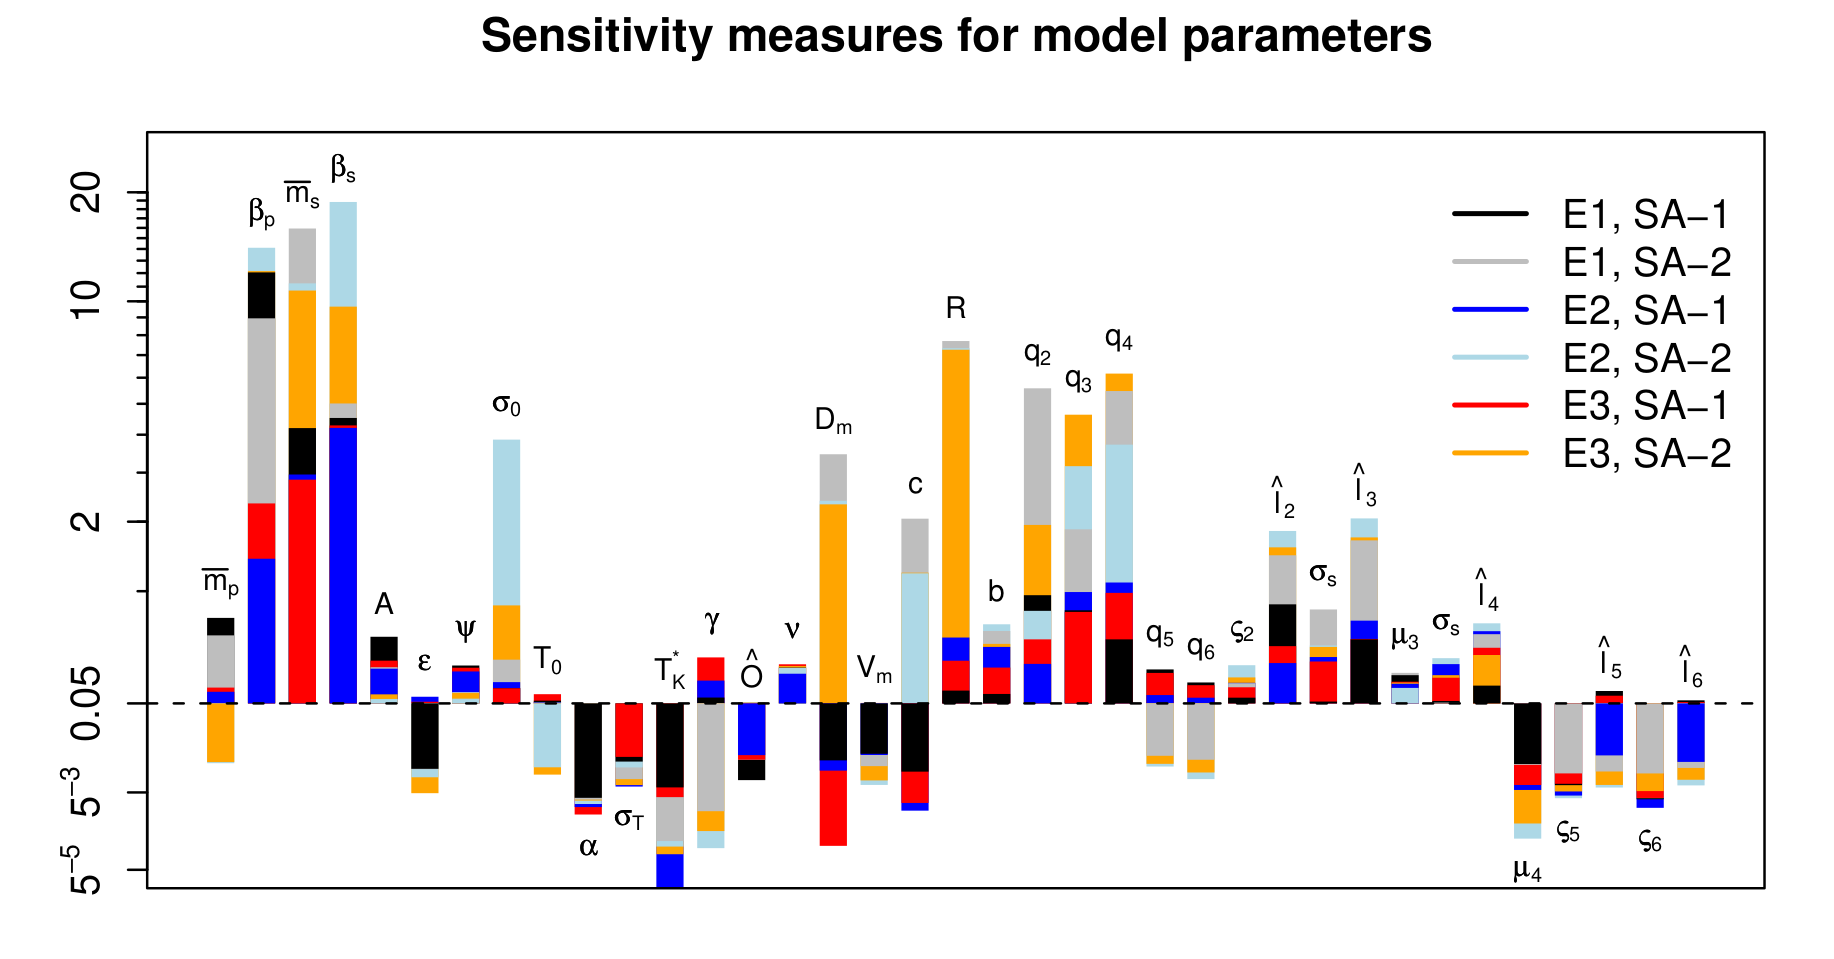
\includegraphics[width=0.95\textwidth]{chapter4/figs/SA.png}
	\caption{Log-scaled measures of sensitivity obtained for estimated parameters from three different experiments, E1, E2 and E3. The values below the dashed line correspond to less than 5$\%$ sensitivity of either predictions (SA-1, i.e., $max{\left|\xi_1,\xi_2\right|}$) or objective function (SA-2, $max{\left|\xi_3,\xi_4\right|}$) to corresponding parameter. From \citet{Senina08}.}
	\label{fig:SA}
\end{figure}


\paragraph{Sensitivity of likelihood function.} The second type of sensitivity analysis examines whether the objective function (which incorporates both predicted and observed data) is sensitive to model parameters. We compare values of negative log-likelihood at some found minimum $\boldsymbol \uptheta^{\dag}$ to those evaluated at the boundaries of the parameter space \citep{Vallino}. We define two further measures of relative sensitivity:

\begin{equation}
 \xi_3(\theta^{\dag}_k)=\frac{L\bar{\text{ }}(\boldsymbol \uptheta^{\dag}+\delta \bar{\theta}_k \cdot \mathbf{e}_k)-L\bar{\text{ }}(\boldsymbol \uptheta^{\dag})}{L\bar{\text{ }}(\boldsymbol \uptheta^{\dag})}, \text{ }
  \xi_4(\theta^{\dag}_k)=\frac{L\bar{\text{ }}(\boldsymbol \uptheta^{\dag}-\delta \underline{\theta}_k \cdot \mathbf{e}_k)-L\bar{\text{ }}(\boldsymbol \uptheta^{\dag})}{L\bar{\text{ }}(\boldsymbol \uptheta^{\dag})}
\end{equation}

\noindent where $\delta \bar{\theta}_k=\bar\theta_k-\theta^{\dag}_k$, $\delta \underline{\theta}_k=\theta^{\dag}_k-\underline\theta_k$ and $\mathbf{e}_k$ is a standard basis vector with 1 in the \textit{k}th  element and 0 elsewhere. \\

%\noindent $\triangleright$ To run this type of analysis, use the option -sa[1] in the command line to execute SEAPODYM. \\

\noindent For both -sa[ ] options, outputs are directly shown on the terminal screen at the end of the simulation and can be recorded in a text file if needed to produce a table (Table ~\ref{table:SA}) or a plot (e.g., Figure ~\ref{fig:SA}). It is recommended that multiple sensitivity tests are run from experiments with different initial conditions, time series of simulation, and estimated values of parameters. This approach will help in detecting persistent patterns, for example, parameters that show consistently low or conversely really high sensitivity, and, hopefully, the reason for such patterns. If the problem cannot be solved, for example, by increasing the period of simulation to include new data or testing a better environmental forcing data set, then the parameter(s) with low sensitivity should be fixed to their best guess or estimate and removed from the optimization.\\


\begin{table}[tbp]
	\centering
		\caption{Example of outputs from the sensitivity analyses.}
		\vspace{0.5cm}
\begin{tabular}{lll}
 N& parameter & relative sensitivity \\
\hline
1& Mp mean exp(0)    & 8.72181      \\
2& Ms mean max(0) 	 & $-1.11762$     \\
3& a sst spawning(0) & 2.54945 e$-10$ \\
4& b sst spawning(0) & 0.00656738   \\
5& a sst habitat(0)  & 3.39733e$-18$  \\
6& b oxy habitat(0)	 & $-1.0208$      \\
7& MSS species(0)    & $-0.070417$    \\
8& nb recruitment(0) & 0.0047095    \\
9& ...	\\
10&...  \\
\hline
\end{tabular}
\label{table:SA}
\end{table}

Note that local sensitivity analyses, although fast and easy to run, only provide a partial representation of observable and non-observable parameters unless the entire parameter space is explored, which is not feasible as it means exploring the entire likelihood hyper-surface in n-dimensional parametric space. Another type of sensitivity analysis, global sensitivity analysis, can be a more practical solution to analyse parameter sensitivity.

\subsection{Global sensitivity analysis}\label{sec:global-sa}

To evaluate the model's sensitivity to its parameters, the SEAPODYM model software also includes  global sensitivity analysis (GSA) based on variance methods \citep{Saltelli, Pianosi}. GSA is performed by computing the first-order (``main effect'') indices measuring the direct contribution from each parameter to the output variance and the total-order (``total effect'') indices measuring the overall contribution from a parameter including its interactions with other parameters. These indices are computed as follows:

\begin{align}
S^F_i = \frac{\mathbf{V}_{\theta_i}[\mathbf{E}_{\theta_{\sim i}}\left(L\bar{\text{ }}|\theta_i\right)]}{\mathbf{V}(L\bar{\text{ }})}; 
{\textbf{ }}
S^T_i = \frac{\mathbf{E}_{\theta_{\sim i}}[\mathbf{V}_{\theta_i}\left(L\bar{\text{ }}|\theta_{\sim i}\right)]}{\mathbf{V}(L\bar{\text{ }})} \label{eq:SA}
\end{align}

\noindent where $\mathbf{E}$ denotes expected value and $\mathbf{V}$ denotes variance, $L\bar{\text{ }}$ is the negative log-likelihood (see next section), and $\theta_{\sim i}$ means varying all parameters but the $i$th. The main and total effect indices are useful to rank and to exclude the non-influential parameters respectively. The $S^F_i$ measures the relative contribution of each parameter to the total output variance, $\sum_i{S^F_i} \leq 1$ for non-linear non-additive models. In other words, when computing first order sensitivity indices, we measure the direct contribution of each parameter (independent from the other parameters) to the output variance. The parameter $\theta_i$ is not influential if and only if the index $S^T_i=0$. Having $S^T_i>S^F_i$ indicates an existing correlation with other parameters. Hence, total-order sensitivity indices measure the overall contribution from each parameter to the output variance, thus including interactions between correlated parameters.

According to \hyperref[eq:SA]{\ref*{eq:SA}}, indices $S^F_i$ can be computed in so-called All-At-a-Time (AAT) SA experiments, that is, randomly sampling all parameters at every model run. The evaluation of $S^T_i$ requires One-At-a-Time (OAT) SA simulations, in which only one parameter is randomly varied in a series of model runs while others are fixed. In order to evaluate model sensitivity to its parameters given the information contained in each type of data, it is good practice to set up three SA simulation studies with model configurations integrating either catch, length frequency, or tag recapture data. As an output function, the code uses the negative log-likelihood functions that are configured for respective type of data.

First, a large number $m$ (usually of order $10^4$) of AAT simulations can be run in parallel for each data type with $n$ parameters shuffled randomly (all at the same time) within their valid ranges, and hence each of $m$ simulation runs has a unique subset of parameters. Second, the subset of parameters $l<<m$ providing the lowest function values in AAT SA simulations can be selected to conduct OAT SA simulations. This allows exclusion of the model solutions that are too far from the optimum and hence unrealistic. Each OAT simulation is configured as a simulation ensemble, starting with one of the $l$ parameter sets of length $n$ and performing $n$ series of runs moving iteratively from the first to the last parameter. For a given parameter, the OAT run performs $k$ simulations with randomly sampled values within a parameter's valid range (one at a time). Note that a number $k=25$ is chosen arbitrarily and can be easily modified in the method's computer code. In addition, the following algorithm has been found efficient to subsequently improve the cost function towards its optimum within OAT simulations, thus combining these sensitivity simulations with the likelihood profiling technique to obtain another useful diagnostic for a parameter estimation problem (section~\ref{sec:like-profiling}). The algorithm consists of starting each $i+1$ OAT iteration with the $i$th parameter being fixed at a value providing the lowest function among a series of $k$ runs. Thus, at every iteration, the OAT is moving towards lower function values, except if the subsequent parameter after being sampled $k$ times could not provide further improvement. In this case, the initial parameter value, corresponding to the best function value in the previous iteration, is retained. Overall, OAT simulations provide $n \times l \times k$ function values and $l \times n$ function profiles of length $k$.

\begin{figure}[H]
\begin{center}
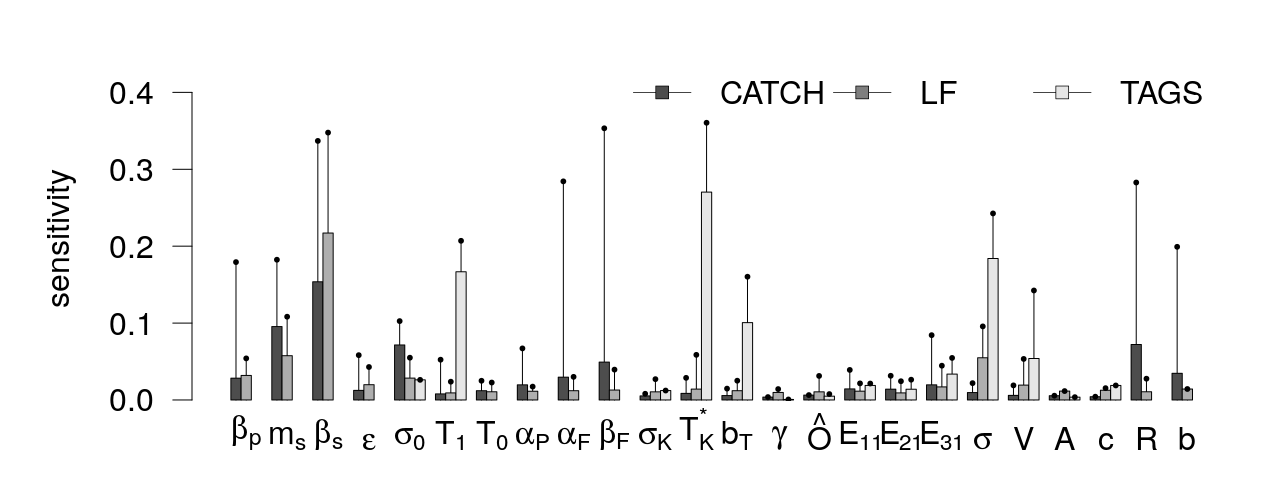
\includegraphics[width=0.925\textwidth]{chapter4/figs/skj-SA-SF-ST}\\
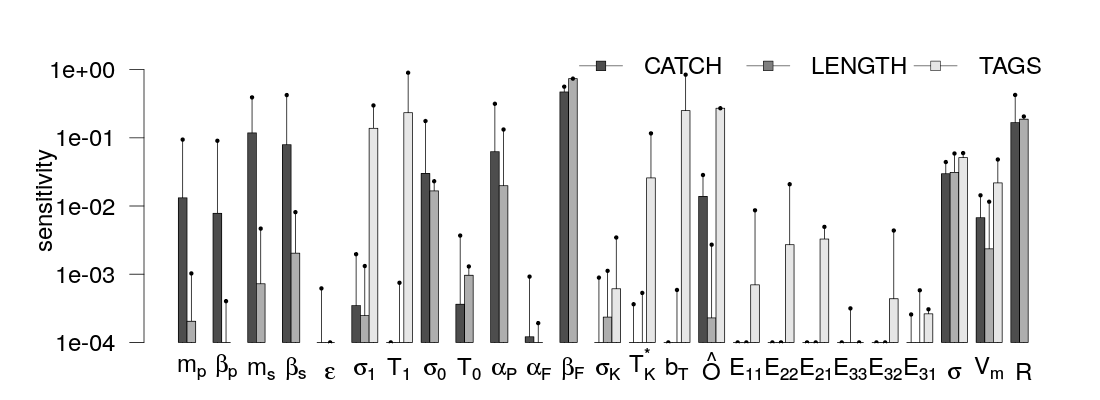
\includegraphics[width=0.9\textwidth]{chapter4/figs/bet-SA-SF-ST}\\
\caption{ Sensitivity indices computed for three negative log-likelihood terms depending on catch, length and tagging data respectively for (top) skipjack tuna\citep*[from][]{Senina20b} and (bottom) bigeye tuna\citep*[from][]{Senina2020c}. Note the linear and logarithmic scales for the results in skipjack and bigeye tuna models respectively.  Bars correspond to the first-order sensitivity showing direct contribution of a parameter to the model output variance, and vertical lines correspond to the total effect sensitivity, including correlations between model parameters (vertical lines). }
\label{SA}
\end{center}
\end{figure}

Figure~\ref{SA} shows the quantitative results of global sensitivity analysis (both AAT and OAT) for skipjack and bigeye tuna. Given the model and observations for these species, integrating fisheries data (catch and length frequency) into the likelihood mainly informs (provides high sensitivity to) the parameters, which influence the reproduction and mortality processes ($m_p$, $\beta_p$, $m_s$, $\beta_s$ and $\alpha_p$, $\beta_F$, $R$ respectively, see Table~\ref{tab:parameters} for description of these parameters). Interestingly, for the bigeye tuna model, the length frequency data principally controls the estimation of recruitment, especially parameters of the spawning habitat index, $\alpha_p$ and $\beta_F$, that drive the seasonality of spatial distribution of recruits. But this is not the case for skipjack tuna, where the LF data provide higher sensitivity to mortality parameters than to those of recruitment. Diffusion and advection rates ($\sigma$, $V_m$) also have  relatively high sensitivity provided by including all three types of data for bigeye tuna, but not for skipjack. For the latter species, the sensitivity to movement rates is mostly driven by tag recapture data. 

Habitat indices parameters, $T_1$, $\sigma_K$, $T_K$, and micronekton multipliers produce almost no or low change in both model outputs with fisheries data. Another habitat parameter, the dissolved oxygen threshold $\hat{O}$ can be estimated well from the bigeye tuna catch data distributions, with its estimation probably being well constrained by strong gradients in the spatial distribution of catches around zones with low oxygen content in the upper mesopelagic layer. For skipjack tuna, primarily occupying the epipelagic layer, which has mostly high oxygen levels, there is a weaker signal for the estimation of this parameter. These two results clearly demonstrate that sensitivity to model parameters is driven by data, their spatio-temporal coverage and the signal they provide to constrain model parameters.

Likelihood profiles for movement parameters, obtained with help of OAT simulations with skipjack and bigeye tuna models are shown in Fig.~\ref{fig:OAT-profiles}. The presence of shape in profiles indicates that the model is sensitive to a given parameter. And the opposite, the flatness and dispersion of profiles, suggests that this parameter is not informed by the data. Profiles for movement rates in both skipjack and bigeye tuna models clearly show the tendency of fisheries data to increase diffusivity and reduce directed movement rates, both contributing to non-zero biomass everywhere in the model domain and low patchiness. The overall pattern is similar in the two models, although there is a slightly increasing trend in length frequency likelihood with increasing values of diffusion rate in the bigeye model and a better defined shape of tagging data likelihood with respect to advection rate, with a minimum located between 0.5~BL/s and 1~BL/s. Overall, integration of tagging data in the models of skipjack and bigeye tuna populations enhances observability of movement parameters while modifying the shape of the likelihood hyper-surface with minimal values towards lower diffusions and non-zero advection rates. See more results and discussion on likelihood profiles in skipjack and bigeye tuna models in recent SEAPODYM studies \citep{Senina20b, Senina2020c, Senina2021}.

\captionsetup[subfigure] {labelformat=empty,labelfont=bf,textfont=normalfont,singlelinecheck=on}
\begin{figure}
\centering
\begin{subfigure}[b]{1.0\textwidth}
\captionsetup{labelformat=empty, justification = raggedright, singlelinecheck = false}   
\caption{a) skipjack tuna}
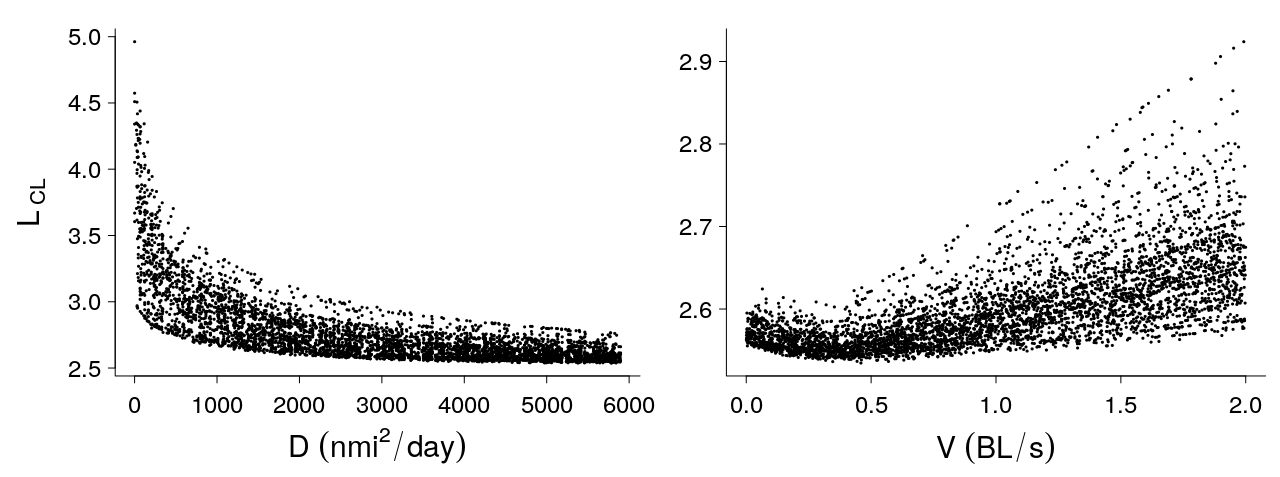
\includegraphics[width=0.6\textwidth]{chapter4/figs/SA-CL-skj}\\
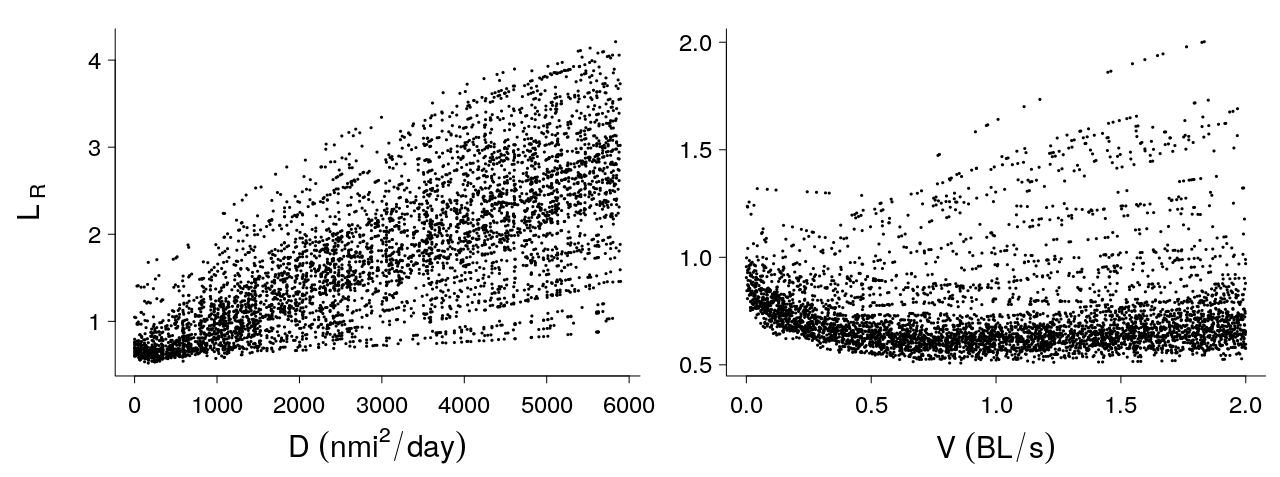
\includegraphics[width=0.6\textwidth]{chapter4/figs/SA-Tags-skj}\\
\end{subfigure}
\begin{subfigure}[b]{1.0\textwidth}
\captionsetup{labelformat=empty, justification = raggedright, singlelinecheck = false}   
\caption{b) bigeye tuna}
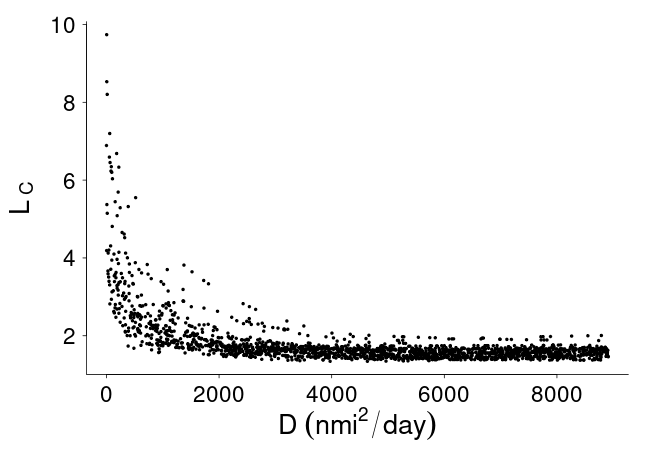
\includegraphics[width=0.3\textwidth]{chapter4/figs/SA-C-sigma-bet}
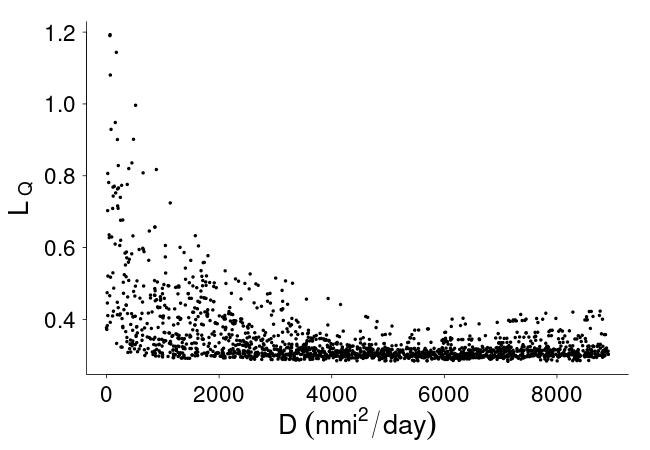
\includegraphics[width=0.3\textwidth]{chapter4/figs/SA-LF-sigma-bet}
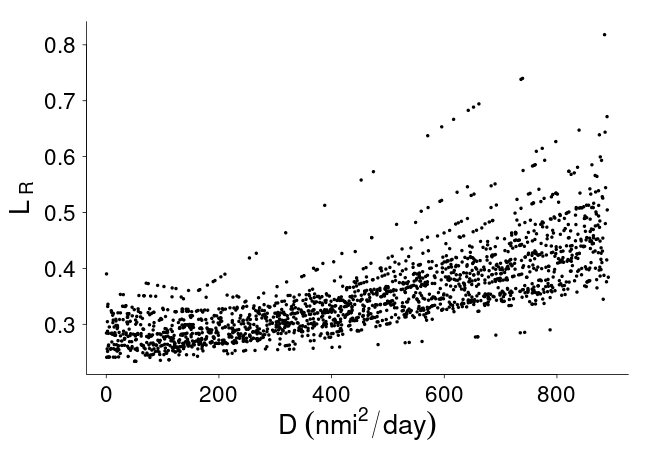
\includegraphics[width=0.3\textwidth]{chapter4/figs/SA-Tags-sigma-bet}\\
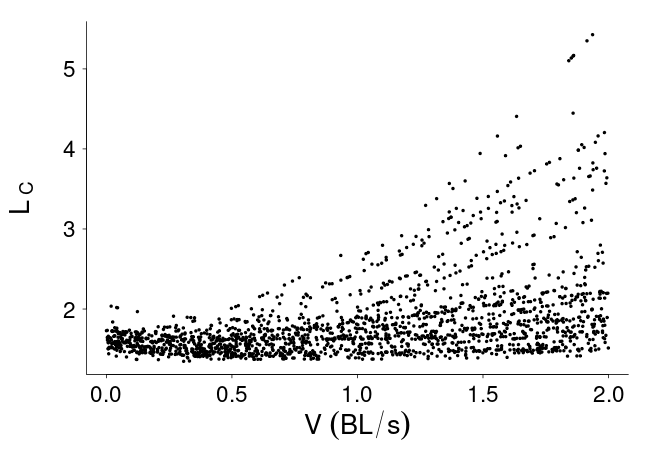
\includegraphics[width=0.3\textwidth]{chapter4/figs/SA-C-V-bet}
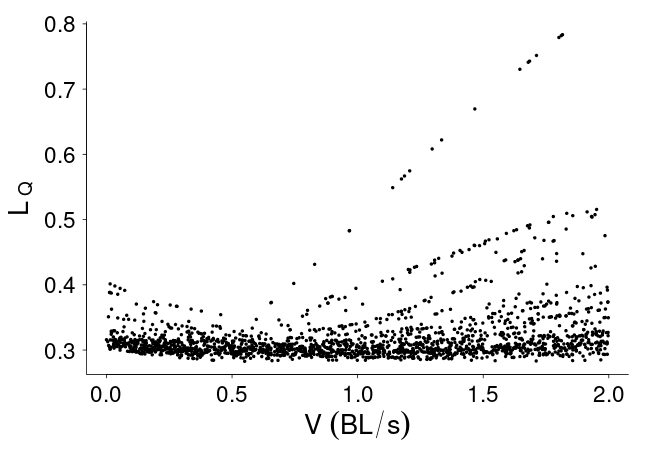
\includegraphics[width=0.3\textwidth]{chapter4/figs/SA-LF-V-bet}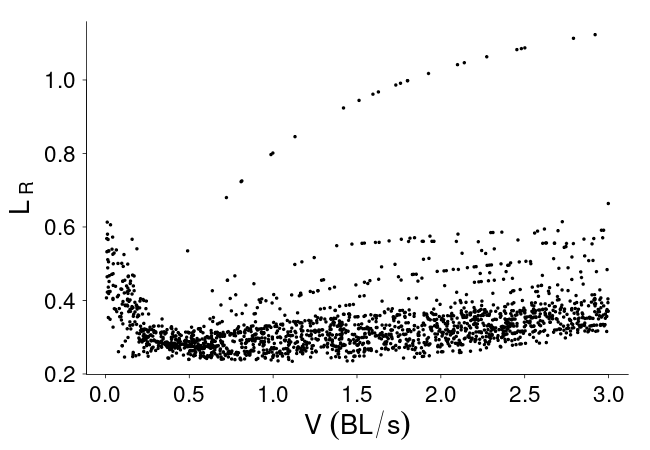
\includegraphics[width=0.3\textwidth]{chapter4/figs/SA-Tags-V-bet}\\
\end{subfigure}
\caption{Likelihood profiles, obtained as a result of OAT simulations for skipjack and bigeye tuna. The scatterplots for the skipjack model correspond to two sets of simulations set up for combined catch and length frequency likelihood and for tagging data likelihood. \citep*[From][]{Senina20b}. For bigeye tuna, each data likelihood term was studied separately \citep*[same results are shown in][]{Senina2020c}. Note, parameter $D$ values correspond to the highest diffusion rate of largest tunas in the population if habitat is null and parameter $V$ is the velocity of density field (in body lengths per second) at highest habitat gradient, that is $\nabla H=1$.}
\label{fig:OAT-profiles}
%\end{center}
\end{figure}


\section{Maximal likelihood estimation method}\label{sec:mle}

To describe spatio-temporal dynamics of fish populations, SEAPODYM relies on parameters that describe the population dynamic rates and provide links between environmental variability and intrinsic dynamic processes such as reproduction, survival and movement. In order to have confidence in model predictions, particularly in the adequacy of the population dynamical responses to environmental variability, we need to combine simulations with quantitative parameter estimation. In other words, we need to inform model parameters, $\boldsymbol\theta$, by fitting the model predictions to the observational data. This is done via use of the maximum likelihood estimation (MLE) method. 

The first implementation of MLE in SEAPODYM is described in \citet{Senina08}. The likelihood function including a new tagging data term is constructed of three observed variables: geo-referenced catch $C_{fKij}$ by fishery $f$, for the time step $K$ and in the observational grid cell $IJ$; length frequency distributions $Q_{fKr}$ in the sampling zone $r$, and the spatial distributions of tag returns $R_{qI^{'}J^{'}}$ in quarter $q$ and the grid cell $I^{'}J^{'}$ of resolution defined for the prediction of tag recaptures. The complete likelihood function of unknown parameters $\boldsymbol \theta$ is computed as follows:
%\begin{linenomath}
\begin{align}
L = \prod_{fKIJ} \left(L(\boldsymbol \theta \mid C_{fKIJ})\right) \cdot \prod_{fKr} \left(L(\boldsymbol \theta \mid Q_{fKr} )\right) \cdot  \prod_{qI^{'}J^{'}} \left(L(\boldsymbol \theta_{\text{tm}} \mid R_{qI^{'}J^{'}} )\right),
\end{align}
%\end{linenomath}

\noindent where parameters $\boldsymbol \theta_{\text{tm}}$ are the subset of parameters of model~\ref{eq:model-1}, which control the dynamics of tag model~\ref{eq:tagmodel}. The MLE is obtained by solving the following constrained minimization problem:

\begin{equation}
\boldsymbol\theta_{\text{mle}} =  \argmin \limits_{\boldsymbol \theta \in (\underline{\boldsymbol \theta},\overline{\boldsymbol \theta})}\left( L\bar{\text{ }} \right)
\end{equation}\label{eq:mle}

\noindent for $L\bar{\text{ }}=-\ln L$. The problem~\ref{eq:mle} is solved iteratively by a quasi-Newton method until the conditions defining a minimum are fulfilled, namely $\frac{\partial (L\bar{\text{ }})}{\partial \boldsymbol \theta} \simeq 0$ and the Hessian matrix is positive definite $\mathbf{H}_{++}$. 

\subsection{Adjoint computer code}\label{sec:adjoint}

Solving the problem~\ref{eq:mle} of function minimization with a gradient method such as a quasi-Newton requires evaluation of the derivatives of the function with respect to each control parameter. In addition, the gradient of the negative log-likelihood, $\frac{\partial (L\bar{\text{ }})}{\partial \boldsymbol \theta}$, must be computed to the same accuracy as the $L\bar{\text{ }}$. In SEAPODYM, we evaluate the function derivatives with help of adjoint computer code, also called reverse mode differentiation code (see e.g. \citet{Griewank}). Direct and derivative code of SEAPODYM is implemented using the objects and memory control of AUTODIF library~\citep{Autodif}, created by David Fournier \citep{Fournier} for automatic code differentiation. This library also provides  the quasi-Newton function minimizer and parameter scaling algorithm for solving the constrained optimisation problem (see below). The use of AUTODIF and its capacity for automatic code differentiation facilitates model developments; however, writing adjoint computer code in order to increase efficiency of computations is always recommended. Thus, the runtime and the memory use can be significantly improved by including appropriate recalculations of the forward model within the adjoint code, rather than storing all the intermediate variables in computer memory. 

When writing new or modifying existing adjoint code, because of the change in the forward code, the resulting analytic derivatives must be verified. This can be done using the AUTODIF derivative check, which uses the central finite difference as the derivative approximation:

\[\frac{L\bar{\text{ }}(\theta_k+h)-L\bar{\text{ }}(\theta_k-h)}{2h}
-\nabla_{k} L\bar{\text{ }}=O(h^2),  
\]

\noindent that is the discrepancy between each gradient component $\nabla_{k} L\bar{\text{ }}$ obtained by analytic differentiation and its finite difference approximation changes parabolically with step $h$, varied from $10^{-6}$ to $10^{-1}$.

\begin{figure}[H]
\begin{center}
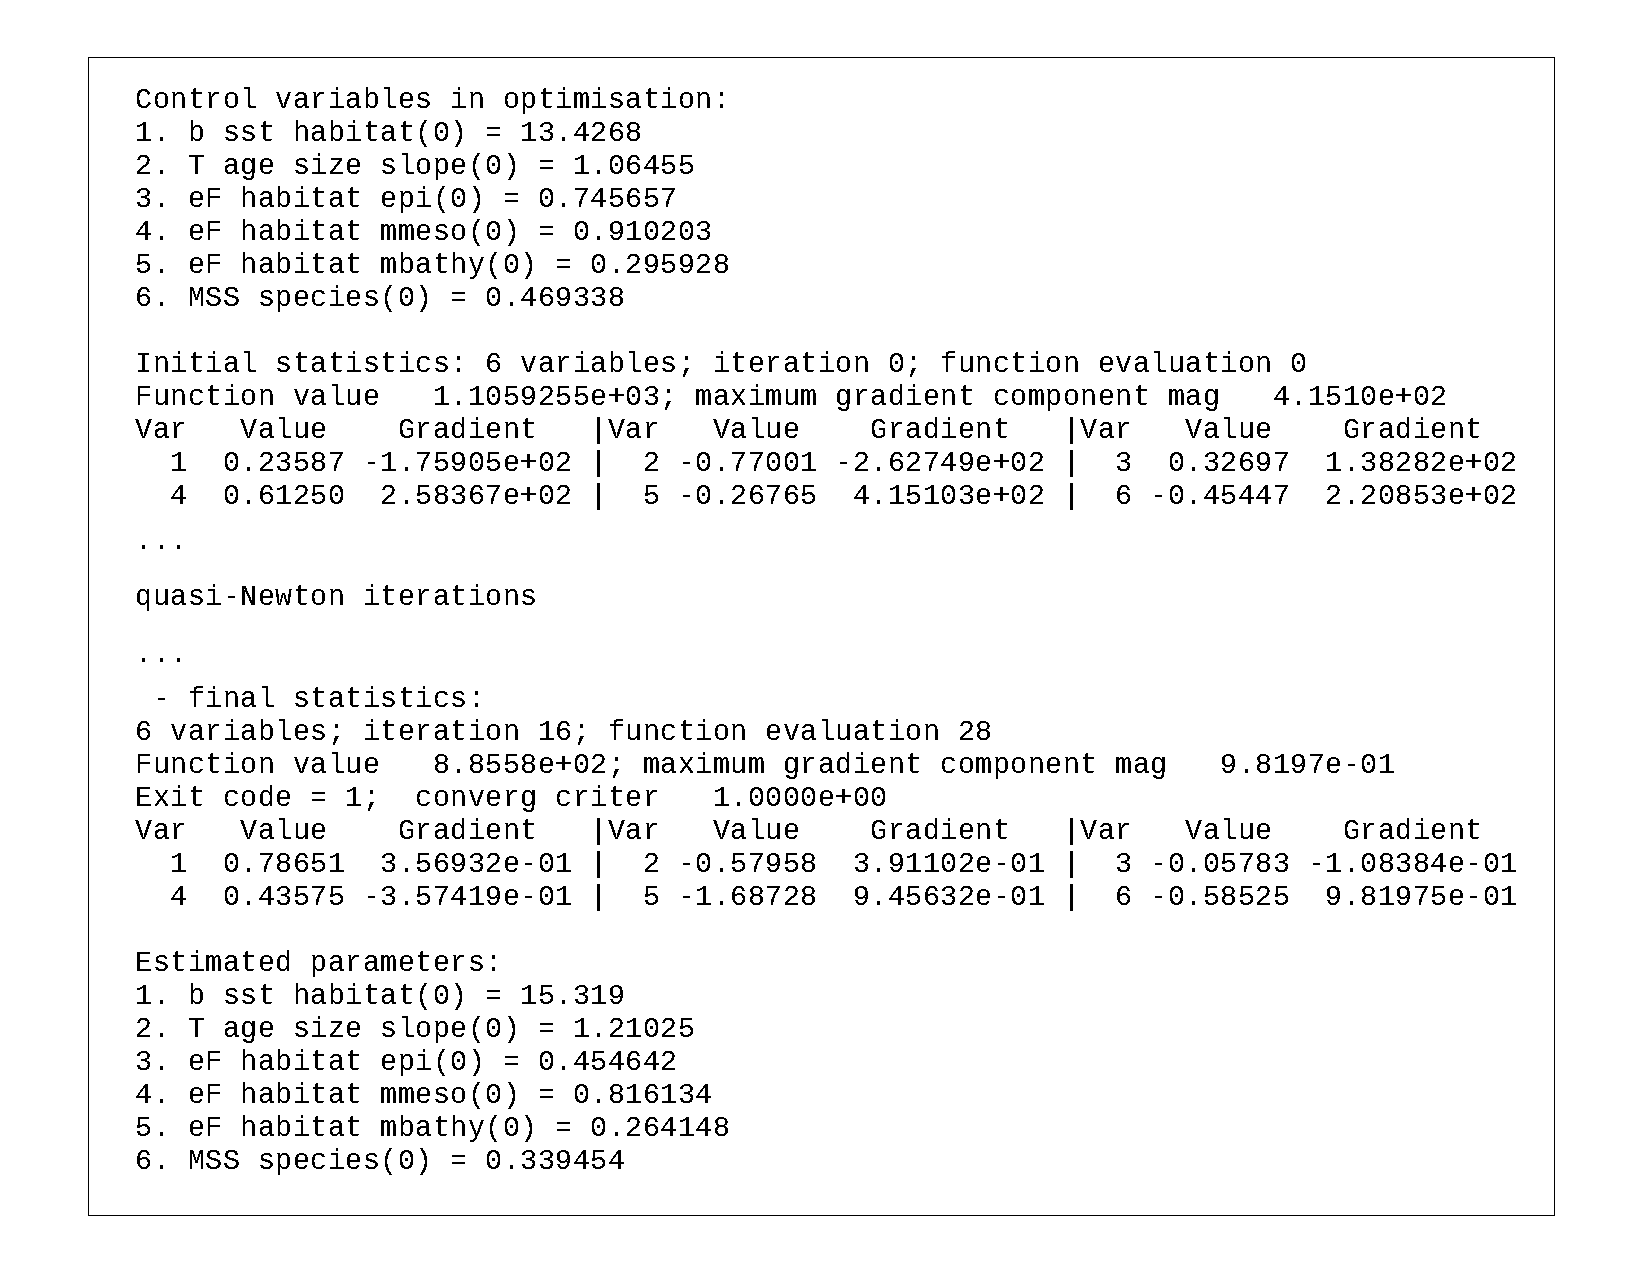
\includegraphics[width=0.925\textwidth]{chapter4/figs/param_scaling}
\caption{Extract from an example optimization run showing the initial and estimated parameters $\theta_k$ and the optimization statistics tables: for each parameter the table provides the value of rescaled parameter $\theta_k'$ and corresponding derivative of the likelihood function.}
\label{fig:param-scaling}
\end{center}
\end{figure}

\subsection{Parameter scaling}\label{sec:parameter-boundaries}

Parameter scaling is done to keep parameters within the allowed range, defined as parameter boundaries. Instead of setting penalties to the boundaries of $\boldsymbol \uptheta$, the AUTODIF library performs a constrained minimization through parameter scaling \citep*[see e.g.,][]{Bard, Vallino}. The latter implies that the optimization routine operates in the unbounded parametric space that is mapped to the bounded one with the transformation:

\begin{equation}
\theta_k=\underline{\theta_k}+\left(\bar{\theta_k}-\underline{\theta_k}\right)\left(1+sin\frac{\pi\theta_k'}{2}
\right),
\label{eq:param-scaling}
\end{equation}

\noindent that is, the variable parameter $\theta_k'$ can vary from $-\infty$ to $\infty$ while $\theta_k$ remains within the imposed  bounds. So, parameter scaling is done prior to optimization, which operates $\theta_k'$ obtained from eq.~\ref{eq:param-scaling} parameters, and at the end of optimization the parameters are rescaled back to $\theta_k$ (see Figure~\ref{fig:param-scaling}). 


\subsection{Likelihood functions in SEAPODYM} \label{sec:likes}

The negative log-likelihood, $L\bar{\text{ }}=-\ln(L)$ to be minimized is the sum of three components: $L_{\scriptscriptstyle  C}^{\bar{\text{ }}}$, the catch data; $L_{\scriptscriptstyle  Q}^{\bar{\text{ }}}$, the length-frequencies data; and $L_{\scriptscriptstyle  R}^{\bar{\text{ }}}$, the tagging data component. These components are described below. For simplicity, let us use notations $f,a,t,i,j,r$ for fishery, age, time, longitudinal, latitudinal and regional indices respectively, knowing that they correspond to data-specific strata defined for each type of observations as described in sections~\ref{sec:integrating-catch}--\ref{sec:integrating-tags}. 

\subsubsection{Catch and CPUE likelihoods}\label{sec:c-like} 

Several functions are implemented in SEAPODYM to account for different statistical distributions of the catch data and hence to define likelihood function components. One frequently used assumption is that observing a non-zero catch event is a rare event and that these observations are described by a Poisson distribution. In this case the likelihood function is equal to the Poisson probability mass function, that is: 

\begin{equation}
L\left(\boldsymbol \uptheta|C^{obs}\right) =
\prod\limits_{tfij}\frac{ {C^{pred}_{tfij}}^{C^{obs}_{tfij}}
e^{-C^{pred}_{tfij}}}{C^{obs}_{tfij}!} {\text {, }} 
\end{equation}

\noindent and the corresponding negative log-likelihood is therefore

\begin{equation}\label{eq:C-like-poisson}
L_{\scriptscriptstyle  C}^{\bar{\text{ }}} =
\sum\limits_{tfij}\left({C^{pred}_{tfij}} - C^{obs}_{tfij} \ln(C^{pred}_{tfij}) + 
\ln\Gamma (C^{obs}_{tfij}+1)\right).  
\end{equation}

The Poisson likelihood is mostly used for the purse-seine fleets targeting the modelled species \citep*[see e.g.,][]{Senina08}. However, this function cannot be used when fishing data contain many zeros, which is often observed for the species that constitutes an accidental catch or is a secondary target for the fleet. In this case, it may be more appropriate to use other distributions, for example, a negative binomial distribution with zero inflation: 

\begin{eqnarray}
L\left(\boldsymbol \uptheta|C^{obs}\right)  = \left\{\!\begin{array}{ll} 
\prod\limits_{tfij}\!\bigg(p_f+(1-p_f)\left(\frac{\beta_f}{1+\beta_f}\right)^{
\frac{\beta_f C^{pred}_{tfij}}{1-p_f}}\bigg) {\text {, if }} C^{obs}_{tfij}=0,\\ 
\prod\limits_{tfij}\!\Bigg(\left(1-p_f\right)\frac{\Gamma\left(C^{obs}_{tfij}+
\frac{\beta_f C^{pred}_{tfij}}{1-p_f}\right)}{\Gamma\left(\frac{\beta_f
C^{pred}_{tfij}}{1-p_f} \right)C^{obs}_{tfij}!}
\left(\frac{\beta_f}{1+\beta_f}\right)^{\frac{\beta_f C^{pred}_{tfij}}{1-p_f}} 
\left(\frac{1}{1+\beta_f}\right)^{C^{obs}_{tfij}}\Bigg) {\text {, if }} C^{obs}_{tfij}>0,
\end{array}\right. & \nonumber \\
&
\label{eq:negbin}
\end{eqnarray}
 
\noindent where the parameters $\beta_f$ and $p_f$, are the negative binomial parameters, the former showing how much variance exceeds the expected value and second is the probability of getting a null observation. Both are estimated in the optimization process. Correspondingly, the negative log-likelihoods are  

\begin{eqnarray}
L_{\scriptscriptstyle  C}^{\bar{\text{ }}} = \left\{\!\begin{array}{ll} 
\sum\limits_{tfij}\!\left( -\ln\left(p_f+(1-p_f)\left(\frac{\beta_f}{1+\beta_f}\right)^{\beta_f\mu_f}\right) \right) 
{\text {, if }} C^{obs}_{tfij}=0,\\ 

\sum\limits_{tfij}\!\bigg( \ln\Gamma(\beta_f\mu_f) + \ln\Gamma(C^{obs}_{tfij}+1)+\ln(\beta_f+1)\left(\beta_f\mu_f + C^{obs}_{tfij}\right) - \ln(1-p_f) \nonumber \\
 \mbox{}- \ln\Gamma(\beta_f\mu_f+C^{obs}_{tfij}) - \beta_f\mu_f\ln(\beta_f) \bigg) 
{\text {, if }} C^{obs}_{tfij}>0,
\end{array}\right. & \nonumber \\
&
\label{eq:C-like-negbinz}
\end{eqnarray}

\noindent where $\mu_f=\frac{C^{pred}_{tfij}}{1-p_f}$. Other available likelihood functions, implemented in SEAPODYM for catch or CPUE data, are derived from truncated Poisson, negative binomial, exponential, Weibull, and log-normal probability distributions. 

Also, if the normal distribution assumption can be made about the catch or CPUE data, then the negative log-likelihood function can be defined as the simple least-square function or as the negative concentrated log-likelihood that is equivalent to the negative log-likelihood for a normally distributed random variable with minimal variance \citep{Fournier}. For example, for the fisheries, for which the catch removal method is used, we choose the normal likelihood profile because the errors are proportional to the modelled biomass and hence can be assumed normally distributed:

\begin{align*}\label{eq:C-like-normal}
L_{\scriptscriptstyle  C}^{\bar{\text{ }}} = \frac{1}{2\sigma^2_C}\sum_{f,t,i,j}\left(C^{pred}_{ftij}-C^{obs}_{ftij}\right)^2.
\end{align*} 

Note that there is not much sense in converting catch predicted with the catch removal method to CPUE, as in this case predicted catch does not depend on fishing effort. Also, the use of observed catch in the catch removal approach may result in $L_{\scriptscriptstyle  C}^{\bar{\text{ }}}=0$ for all $fiij$ if there is always enough biomass to support the observed catch (see eq.~\ref{eq:CR}). Therefore, another likelihood term, allowing the biomass constraint, is necessary (see section~\ref{sec:beta-like}). 

\subsubsection{Length frequency likelihoods}\label{sec:lf-like}

Note that proportions of catch-at-age given by eq.~\ref{eq:LF} do not depend on fishery-specific catchability coefficients. Hence, using only LF data in the likelihood, these parameters cannot be estimated. Two functional forms of likelihoods for LF data are implemented in SEAPODYM, both based on the assumption of normal distribution of the small-scale LF observations. The first function gives the following contribution from length frequency data to the negative log-likelihood:

\begin{equation}\label{eq:lf-like1}
L_{\scriptscriptstyle  Q}^{\bar{\text{ }}} = \frac{1}{2\sigma^2_Q}\sum\limits^{tm}_{t=1}\sum\limits^{n_f}_{f=1}\sum\limits^{n_a}_{a=1}\sum\limits^{n_r}_{r=1}
\left(Q^{pred}_{fatr}-Q^{obs}_{fatr}\right)^2,
\end{equation} 
\noindent where the proportion at age $a$ in the catch computed from the observed length frequency data is $Q^{obs}_{fatr}=\frac{N^{obs}_{fltr}}{\sum_l N_{fltr}}$, $l \in \left[\underline{l_a},\overline{l_a}\right)$. $N^{obs}_{tflr}$ is the number of fish of length $l$ in region $r$ that belongs to the cohort of age $a$. The variance $\sigma^2_Q$ is assumed to be a constant value set up in the computer code, which cannot be estimated.

The second type of LF likelihood function uses the formulation proposed by \citet{Hampton-Fournier} for the fitting to the length frequency data. It is called the robustified likelihood:

\begin{align}\label{eq:lf-like2}
L_{\scriptscriptstyle  Q}^{\bar{\text{ }}} = 0.5\sum\limits_{f,t,r} log\left(2 \pi \left(\xi_{ftr}+\frac{1}{I}\right)\right)+		I\sum\limits_{f,t} log(\tau_{ft}) + \sum\limits_{f,a,t,r} \frac{\left(Q^{\text{obs}}_{fatr}-Q^{\text{pred}}_{fatr}\right)^2}{2\tau^2_{ft} \left(\xi_{ftr}+\frac{1}{I}\right)},
\end{align}

\noindent where the constant $\xi_{ftr}=Q^{obs}_{ftr}(1-Q^{obs}_{ftr})$, $\tau_{ft}=\frac{P}{min(1000,S_{ft})}$ and $I$ is the number of size intervals in the original samples (before redistribution to the model age structure). The term $min(1000,S_{ft})$ embodies an assumption on the maximal sample size to be considered accurate and the constant $P$ assigns how much the variance of the LF sample is greater than that of the truly random sample of a given size. See more details on this likelihood in \citet{Hampton-Fournier}.

\subsubsection{Tag recapture likelihoods}\label{sec:tag-like}

The contribution to the negative log-likelihood function from the tag recaptures data can be defined based on the assumption of the number of tag recaptures being normally distributed:

\begin{align}\label{eq:tag-like1}
L_{\scriptscriptstyle  R}^{\bar{\text{ }}} = w_R \sum_{q,I,J}\left(R^{pred}_{qIJ}-R^{obs}_{qIJ}\right)^2,
\end{align} 

\noindent where $w_R$ is a constant allowing equal weighting between the different likelihood terms, $R^{pred}_{qIJ}$ and $R^{obs}_{qIJ}$ are the number of tag recaptures predicted and observed respectively in quarter $q$ and coarse resolution cells $IJ$. Alternatively, the log-normal likelihood can be defined based on the assumption that tag recapture data are log-normally distributed. Since the tag recapture data may contain true zeroes, they can be accounted for by adding a small constant to both predictions and observations, hence leading to the following contribution to the negative log-likelihood:

\begin{align}\label{eq:tag-like2}
L_{\scriptscriptstyle  R}^{\bar{\text{ }}} = w_R \sum_{q,I,J}\left(\ln\left(R^{pred}_{qIJ}+c\right)-\ln\left(R^{obs}_{qIJ}+c\right)\right)^2,
\end{align} 

\noindent where the constant $c<<1$ is currently set up directly in the computer code. 

\subsubsection{Biomass constraint}\label{sec:beta-like}

Another objective related to the use of catch removal method is to estimate the minimal population stock with an age and spatial distribution that would support the observed catches given the selectivity of fishing gears. By definition in this method, predicted catch in the grid cell is exactly the observed catch if the modelled biomass is sufficient to sustain it (\hyperref[eq:CR]{eq. \ref*{eq:CR}}). In this case the observed catch is simply subtracted from the biomass, and the predicted catch is equal to the observed. Therefore, predicting biomass above the observed catch in all strata is optimal with this method, but increasing the biomass to achieve zero error may lead to an overall model solution that is totally unrealistic. On the other hand, the use of such predictions in the optimization provides the observability of model parameters from the grid cells where the predicted biomass is lower than the observed catch. In this case, the predicted catch is equal to the available biomass, the biomass becomes zero after catch removal and the contribution to the likelihood becomes non-zero. In order to prevent an overestimation of the biomass and to facilitate the convergence towards a realistic solution with the minimal biomass supporting the observed catch, the likelihood must include one additional term allowing the minimization of the total biomass to the lowest possible levels. Fitting the predicted to the observed catch then means reducing the local discrepancies in the case of the lack of biomass. This can be achieved by adding the following contribution to the negative log-likelihood:

\begin{align}\label{eq:beta-like}
\beta = \left(\frac{1}{n_t}\sum_{atij}\left(N_{atij}W_a\Delta x_i \Delta y_j\right) -
\overline{B}\right)^2,
\end{align}

\noindent where $n_t$ is the number of model time steps in the likelihood computation, $W_a$ is the mean fish weight at age $a$ and $\overline{B}$ is the mean stock biomass, assumed to be minimal for the whole domain or a specific part of it. Hence, in the case of using fisheries accounted with observed catch only, the function to be minimized becomes $L\bar{\text{ }}=-\ln L +\beta$, where $L$ includes at least two other likelihood terms, for example, effort-based catch for selected fisheries and LF likelihoods, or the LF and the tagging data likelihoods. Given the poor observability of model parameters from catch data (Figure~\ref{fig:OAT-profiles}), it is essential to use data with good spatial and species life history coverage to estimate those reproduction, mortality, habitat and movement parameters that control spatial distributions of population density at different ages. 

The biomass $\overline{B}$ can be chosen empirically in a series of optimization experiments so that at any time step and grid cell the exploited biomass $\sum_{af} \left(s_{af} N_{tij} W_a \Delta x_i \Delta y_j\right) \geq 0.8 C^{obs}_{tij}$ , where $s_{af}$ is the fisheries selectivity. Ideally the level of biomass should always be higher than the observed catch; however, up to 20\% local errors can be allowed because of biases in the physical forcing, the errors in the fishing data and the coarse spatial resolution of the numerical model. 

\section{Parameter estimation workflow}\label{sec:fmin}

The search for a best set of parameters, corresponding to the global minimum is not a trivial task within complex non-linear models, and requires lots of optimization experiments that differ in the configuration of model structure, the data to be used in the likelihoods, likelihood definitions, the set of variable and fixed parameters and finally the initial parameter values. Here are some brief statistics of optimizations undertaken to achieve the MLE solutions described in \citet{Senina20b} with catch and length (CL) and catch, length frequency and tag recapture data (CLT) for skipjack tuna. About 40 optimization experiments with CLT likelihood, corresponding to $\approx 15,000$ function evaluations (FE) in total, 25 optimizations for CL ($\approx 6000$ FE) and 310 optimizations ($\approx 150$ FE by optimization on average) with tagging likelihood only. Every parametrisation obtained as a result of function minimization, has to be analysed, the parameter estimates confronted with the best available knowledge about the modelled species, and the fit and errors and biases evaluated. 

This section describes the parameter estimation workflow, covering some aspects of the optimization experiment set-up and available tools for troubleshooting and additional model and method analyses in case if the method does not converge or if the MLE solution is not satisfactory.

\subsection{Problem dimensionality and memory control}

First, to maintain the time of computation at a reasonable level, it is necessary to find a balance between the number of observations, the size of the domain, the spatial and temporal resolution, and the extension of the time series used in the optimization experiment. The dimensionality of the optimization problem affects the runtime and the amount of memory needed to store all intermediate variables for adjoint calculations. 

The AUTODIF library controls memory allocation. Three buffers are declared with their sizes defining the memory for the variables dependent on parameters $\boldsymbol\theta$, called \textit{dvariables}, and for their derivatives. The names of these buffers in SEAPODYM are: {\ttfamily gs\_var\_buffer} -- allocated to store \textit{dvariables} and all AUTODIF objects declared in the code, {\ttfamily cmpdiff\_buffer} -- to store the gradient information as well as intermediate variables used by the adjoint code for computing derivatives, and {\ttfamily gradstack\_buffer} -- to store the information necessary to calculate derivatives via automatic differentiation. Note that since the adjoint versions are written for most SEAPODYM functions to compute analytical derivatives, the exceptions are the final likelihood operators, the third buffer is very small compared to {\ttfamily cmpdiff\_buffer}. See the AUTODIF documentation~\citep{Autodif} for more details on the format and the use of these buffers. 

The amount of memory is set up in the program code. The function returned by {\ttfamily main} begins with passing the buffer sizes to a gradient structure object of AUTODIF library:

\vspace{0.35cm}
{\ttfamily
\indent	gradient\_structure::set\_GRADSTACK\_BUFFER\_SIZE(gradstack\_buffer);\\
\indent	gradient\_structure::set\_CMPDIF\_BUFFER\_SIZE(cmpdif\_buffer);\\
\indent	gradient\_structure gs(gs\_var\_buffer);\\
}

\noindent There are two different default buffers settings -- for simulation and optimization modes. In a simulation mode, the default settings allow running the basin-scale coarse resolution numerical models for populations with relatively long lifespan, e.g., describing monthly dynamics of an exploited population with up to 181 monthly age classes and 20 fisheries on a 2$^\circ$ grid over Pacific Ocean domain. The model with this maximal configuration allocates 4 Gb of RAM in a simulation mode. To run optimizations, the default setup admits model configurations of much lower dimensions, also limited in number of time steps in simulation. The example of configuration above, but with only 85 monthly age classes (e.g., see the parfile for Pacific bigeye tuna population model in Appendix~\ref{sec:appendix-parfile}) and simulation time of only ten years yields maximal memory allocation during optimization run,  using 26 Gb of physical memory. Hence all configurations with smaller dimensions are safe for running the numerical model with default memory settings. 

It is possible, although not recommended due to long runtimes, to run optimizations for higher dimension configurations. It is important that the size of the buffers is set up as large as required to store all information in the physical memory during the optimization runs. Otherwise, if the size of the buffer is insufficient, the program will write its contents to the hard disk, into files cmpdiff.tmp, gradfil1.tmp and gradfil2.tmp, which will considerably slow down the program execution. The indicator of correct configuration of the gradient structure buffers is that these temporary files have size 0. Note that in a case of insufficiently large {\ttfamily gs\_var\_buffer} or {\ttfamily cmpdif\_buffer}, the program will exit printing corresponding error message. To increase the size of the buffer(s) manually, the long integer value can be passed via the command line options while launching seapodym:

\vspace{0.2cm}
{\ttfamily
\indent \textbf{seapodym} [\textbf{-option}] [\textbf{-mv} \underline{gs\_var\_buffer}] [\textbf{-mg} \underline{gradstack\_buffer}]  \linebreak 
\indent \hspace{1.8cm} [\textbf{-mc} \underline{cmpdif\_buffer}] parfile.xml\\
}
\vspace{0.2cm}
 
\noindent with the choice of {\ttfamily \textbf{option}} is described in section~\ref{sec:firstrun}. 

During optimization, the SEAPODYM software writes the optimization report file in the run directory named ``optim.rep''. It is updated upon each successful iteration. This file contains the intermediate parameter values (without scaling), the function value and the maximal gradient as well as the execution time per function evaluation. This file is particularly useful for estimating the total runtime of the optimization experiment. The rule of thumb is to multiply the number of parameters by three to get the total number of iterations.

\subsection{Likelihood configuration}

The available likelihood configuration parameters are all listed in Chapter~\ref{ch:configurations}, section~\ref{sec:config-likelihood}. The choice of the likelihood terms is done by setting the flags {\ttfamily frq\_likelihood}, adding or removing the term~\ref{eq:lf-like2},  {\ttfamily tag\_likelihood}, adding or removing the term \ref{eq:tag-like1}, and the flag {\ttfamily stock\_likelihood} to control the term~\ref{eq:beta-like}. Note that catch likelihoods (defined by fishery) are always active and only the types of these likelihoods can be selected in the configuration parfile. However, it is possible to exclude certain fisheries from the likelihood computation via modification of vector {\ttfamily mask\_fishery\_likelihood}. The type of catch variable, that is the use of catch or CPUE in the likelihood, can be set up via flag {\ttfamily like\_c\_cpue}. The average stock value as well as the region over which this value is computed can be configured in the parfile (see {\ttfamily mean\_stock\_obs} and corresponding regional parameters).

Finally, it is possible to solve optimization problem with tagging data only. This is activated by the flag {\ttfamily tag\_likelihood\_only}. In the latter case only model~\ref{eq:tagmodel} will be solved for the tagged cohorts defined in the input tagging data files, which are also provided in the parameter file (see Appendix~\ref{sec:appendix-parfile}).
 
\subsection{Initial conditions}

We distinguish between the initial conditions of optimization, that is the initial parameter values and the initial conditions of model~\ref{eq:model-1}, that is the model's initial state vector. 

\subsubsection{Initial parameter values}

It is important to configure and run multiple optimization experiments starting from different initial parameter values. This method uses what are called ``jitter'' optimization runs. The approach of perturbing the model parameters and restarting the experiment prevents the model converging towards the local minima, although it is not a rigorous method to ensure that the found solution is a global minimum. For the latter, it is necessary to use the global optimization methods such as simulated annealing \citep{Matear} or a genetic algorithm. 

\subsubsection{Initial state vector}

Regarding the initial distributions of population density, they may also greatly influence parameter estimation as the model numerical solution depends on them. The sensitivity to the initial conditions can be evaluated by running several optimization experiments starting from different initial states. The influence of initial conditions on the results of minimization can be reduced by skipping the first predictions from being used in the likelihood computation. The number of time steps to skip is configured by the parameter {\ttfamily nb\_step\_to\_skip} in the parfile. The simplest way is to exclude the number of time steps corresponding to the age at 50\% maturity of modelled species, that is the time necessary for the new larval production to enter the mature stock and the mature stock to be redistributed according to the currently estimated parameters driving the spatial dynamics. Note that it might be impractical to skip a long period and hence a large number of observations in the case of long living species with late maturity. Thus, realistic assumptions on the population abundance and availability of spatial distributions from previous optimizations might be necessary.


\subsection{Role of environmental forcing}

The parametrization of SEAPODYM is highly sensitive to ocean forcing. Therefore, a realistic ocean forcing, that is, based on observations, is necessary to drive the population dynamics. Realistic physical and biogeochemical variables are necessary to explain the observed variability within the large datasets of tuna catches and length distributions, which in turn reflect changes in fish abundance due to both fishing and the impact of environmental variability, including ENSO (El Nino southern oscillation) events.

Constraining the population dynamics of SEAPODYM, environmental data can be viewed as ``fixed'' parameters, and it is essential that these parameters are ``optimal''. However, environmental forcing is itself modelled data and has biases. In addition, optimization experiments are usually configured with the coarse spatial resolution model, which is characterized by weak representation of ocean circulation and subsequent biases in primary production and micronekton densities. For example, the correct temperature variability is of primary importance to determine seasonal spawning or feeding migrations. A model that is unable to adequately describe the seasonal migrations because the temperature seasonality and spatial structure have biases in the geographic area being the population spawning or feeding ground or the area of migration route, will tend to bias parameters of habitat indices and to extend the overall biomass distribution, if data from a corresponding geographic area will be used in function minimization. Consequently, it is advisable to exclude from the likelihood calculation the data associated with the complex current systems if the forcing data underestimates them, or the data showing highly heterogeneous patterns if the model spatial resolution does not allow reproducing them. Note that excluding fisheries from the likelihood function does not mean excluding them from the computation of fishing mortality. However, each case should be examined in the context of its impact on both the maximum likelihood estimation and the local mortality rates. 

\subsection{Identical twin experiments}\label{sec:twin-experiments}

Demonstrating that a solution found by numerical optimization is a global solution and not a local minimum is a difficult and well-known problem in all non-linear optimization problems and data assimilation. Evaluation of the uniqueness of the estimated parameters is challenging because of the complexity of the ecosystem model, the high dimension of the objective function and scarcity of available observations \citep{Robinson,Vallino}. Unfortunately, one cannot prove that minima found by the gradient descend method are not local minima. Considering the computer time to perform one experiment, it is also unrealistic to envisage an exhaustive study that would allow us to conclude that computed solutions are global. It is possible, however, to evaluate the reliability of the solutions by conducting so-called ``identical twin experiments''. They can  verify that both the model and the method allowed the estimation of chosen parameters using the available number of observations. These tests consist of estimating parameters from artificial data series constructed from predictions given by the model. If optimization works well with the model and experiment set-up, then after sufficient perturbation of optimal parameters we should be able to retrieve them, because they determine a known a priori solution represented in the artificial data series. 

Configuring and running the twin experiments with SEAPODYM  can be done in the following steps:
\begin{itemize}
 \item[-] run a simulation with selected set of parameters;
 \item[-] using the model predictions for catch, length and tag recapture data, create an artificial data set, with or without adding noise to the data, format the model outputs as the input data;
 \item[-] perturb the initial values of the parameters to be estimated in the parameter file;
 \item[-] run SEAPODYM in the optimization mode until convergence to the MLE solution;
 \item[-] use the optim.rep output file to check the result and produce plots. \\
\end{itemize}

\begin{figure}[H]
	\centering
		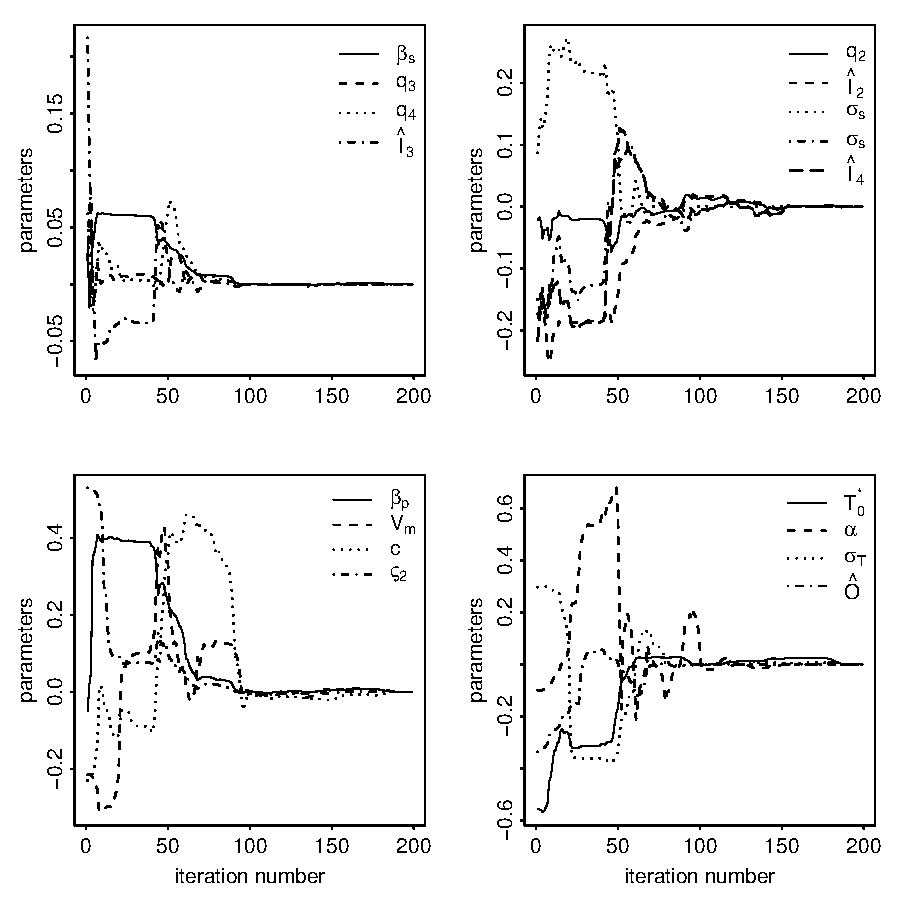
\includegraphics[width=0.9\textwidth]{chapter4/figs/twin_E2}
	\caption{Evolution of control parameters during twin data experiment conducted for the artificial data simulated with skipjack tuna model configuration. Parameters are grouped by their sensitivities in descending order. \citep*[From][]{Senina08}.}
	\label{fig:twinE2}
\end{figure}

Twin experiments conducted for the skipjack tuna application \citep{Senina08} have shown that the control parameters were successfully recovered with small relative errors $\varepsilon< 0.001$ due to the computer round-off error. The evolution of the parameters during the minimization process can be plotted (see figure ~\ref{fig:twinE2}) to illustrate how quickly the parameters were recovered, and which parameters are the most difficult to correctly estimate. \\

\subsection{Two-dimensional projection of likelihood function}\label{sec:like-profiling}

Sometimes it is useful to explore the likelihood function visually, plotting different projections of likelihood hyperspace over the pair of selected parameters. This may give a clue about the observability of a certain parameter, whether the boundaries of the parameter should be modified, how the penalty function changes the shape of the likelihood, and so on. Plotting the cost function is also a simple way to visualize the localisation of the solution found. For example, the likelihood function can have multiple minima and the likelihood projection plot can reveal the local minimum problem and help to navigate the minimization experiments further. Figure~\ref{fig:hyperplot1} illustrates an example of the the cost function having two local minima, with one local minimum around 10$^\circ$C for preferred habitat temperature, which is totally unrealistic for yellowfin tuna. 

\begin{figure}[H]
	\centering
		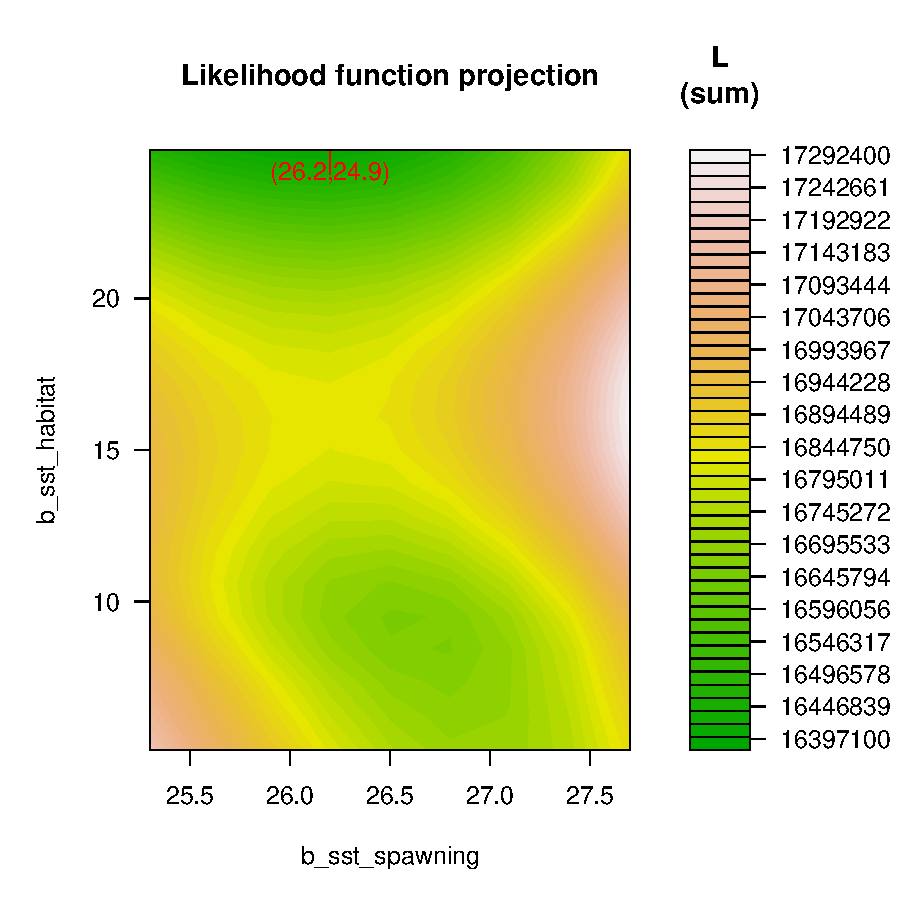
\includegraphics[width=0.8\textwidth]{chapter4/figs/Fig_hyperplot_yft_2mins}
	\caption{Likelihood projection over two habitat parameters in the yellowfin tuna model.}
	\label{fig:hyperplot1}
\end{figure}

Besides, the numerical instability problems, or the high-mode non-linearity of model solutions, and/or noisy observations can result in abrupt, spiky surfaces of the cost function and hence impede the convergence of the minimization method. The two-dimensional likelihood profiling is activated by execution option ``-p'' (see Chapter~\ref{ch:configurations}, section~\ref{sec:profiling-run} for details on configuring and running these simulations).

\subsection{Correlations between parameters}\label{sec:par-correlations}

To be well determined, the model parameters, i.e. control variables in optimization, must be independent. However, correlation between model parameters is a common issue. For example, increase of the larval recruitment rate on one side and increase of the predation mortality of larvae on the other can provide the same number of recruits, and hence the simultaneous estimation of these two parameters can lead to biased estimates of the total population size. If parameters are correlated, the minimization procedure will increase the number of iterations, leading to an overall increase in the computational time. Establishing correlations between all model parameters can help reduce the number parameters to enable their successful estimation, while fixing their correlated pairs at reasonable and meaningful values.

Correlation coefficients between pairs of estimated parameters can be derived from the off-diagonal elements of the error-covariance matrix, which is the inverse of the second-order derivative, or Hessian, matrix:

\begin{align}\label{eq:covarmat} 
\mathbf{C}=\mathbf {H}^{-1} & \mbox{, with } \mathbf H=\frac{\partial^2 L\bar{\text{ }}}{\partial \theta_i \partial\theta_j}, \text{ } i,j=1,2,...,n
\end{align}

\noindent where the Hessian matrix $\mathbf{H}$ must be evaluated with $\boldsymbol\theta_{\text{mle}}$. Numerically, the Hessian matrix is approximated in SEAPODYM with central finite difference using first derivatives exactly evaluated by adjoint calculations. It is obtained by running the SEAPODYM software with option ``-h'' and the parfile with MLE parameters (see Chapter~\ref{ch:configurations}, section~\ref{sec:hessian-run} for more details on the outputs). 

It is desirable to study the correlations between parameters ahead of optimization, although in practice it is never the case because the Hessian has to be evaluated at the point of minimum to ensure the good precision by finite difference method. On the other hand, it makes little sense to do optimization with all data first, hoping to correctly estimate model parameters without knowing that they are independent. The best practice is to use the twin experiment configurations with a priori known solutions and to perform correlation analysis.

\begin{figure}[H]
	\centering
		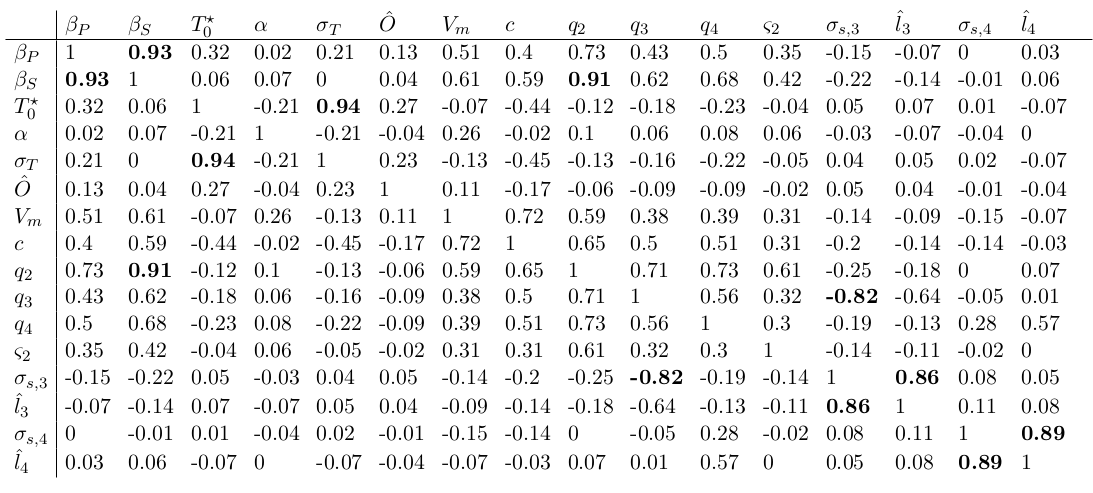
\includegraphics[width=1.0\textwidth]{chapter4/figs/cor-table}
	\caption{Correlation coefficients between skipjack tuna model parameters, showing high correlations between 1) predation, $\beta_p$, and senescence, $\beta_s$, mortality rates, 2) catchability of pole-and-line fishery, $q_2$, and senescence mortality rate, 3) parameter $\sigma_T$, defining thermal preference range, and the optimal temperature for spawning, $T^{*}_0$ as well as between some catchability and selectivity parameters \citep*[From][]{Senina08}.}
	\label{fig:cor-table}
\end{figure}


\section{Error analysis}\label{sec:uncertainty}

The current SEAPODYM version allows computation of the parameter estimation error in the vicinity of the found minimum. Obviously, this approach evaluates whether the estimated parameters are well determined at the minima detected by the minimization routine, which may not be a global minimum. That is why it is important to perform jitter optimization runs, perturbing the model parameters and restarting the experiment to verify that the model has converged towards the minimum of the experiment. Then, to get the parameter estimation error, we compute the variance of the estimated parameters from the error-covariance matrix~\ref{eq:covarmat} obtained from the Hessian matrix. Note that the Hessian matrix $\mathbf{H}$ must be evaluated with $\boldsymbol\theta_{\text{mle}}$, that is at the minimum of the negative log-likelihood function.

The diagonal elements of the variance-covariance matrix $\mathbf{C}$ provide estimates of the variance of the optimal parameters. From the variance we derive the standard deviations, providing the measure of uncertainty on the parameters estimates. Small uncertainty is an indicator that the parameter was well estimated from observational data given the found minimum. Large uncertainties obtained in this error analysis are good indicators of poorly determined (poorly observed) parameters. \\

\section{Model validation}\label{sec:validation}

The validation of model solutions can be done via the following steps:

\begin{itemize}
\item evaluation of the improvement of the fit to the data due to optimization; 
\item analysis of model dynamics under estimated parameter values; 
\item measuring the fit with the optimal solution to an independent dataset. 
\end{itemize}

To measure how well the model describes the data used in optimization and how well it fits to the independent data, we can use three statistical metrics:  (1) the coefficient of determination $r^2$ (squared Pearson correlation coefficient), reflecting the percentage of predicted variability that is consistent with observations; (2) the standard deviation ratio $\sigma_{rel}$, that is the ratio between standard deviations of model predictions and those of data; and (3) the normalised mean square error, $\text{NMSE}$ (\hyperref[eq:r2]{eqs. \ref*{eq:r2}--\ref*{eq:nmse}}). The best score is 1 for $r^2$ and SDR, and 0 for NMSE. Note, these metrics can be computed and compared between different model predictions for: (1)$R$ -- tag recaptures, (2) $C$ -- catch predicted by the catch removal method, and (3) $EC$ -- catch based on the fishing effort. Note that to compute the scores for $EC$, the catchability parameters must be estimated for those fisheries that are used in optimization with the catch removal method.

Let $x$ denote the set of observations and $y$ the model predictions of length $N$. Statistical metrics are computed and plotted on a Taylor~\citep{Taylor} diagram (Fig~\ref{fig:taylor}) as follows:

\begin{align}
& r^2 = \frac{\left(\frac{1}{N}\sum\limits_{i=1}^N{ (x-\bar{x})(y-\bar{y})}\right)^2}{\sigma^2_x \sigma^2_y} \label{eq:r2} \\
& SDR = \sigma_y/\sigma_x\\
& NMSE = \frac{\left(\frac{1}{N}\sum\limits_{i=1}^N \left((x-\bar{x})-(y-\bar{y})\right)^2\right)^{\frac{1}{2}}}{\sigma_x}\label{eq:nmse}
\end{align} 

\noindent where $\sigma_x$ and $\sigma_y$ are the standard deviations of observations and predictions respectively, $\bar{x}$ and $\bar{y}$ are the means, and $\text{NMSE}$ is the centred root-mean-square error normalized by the standard deviation of the observations.

\begin{figure}[H]
	\centering
	    \vspace{1cm}
		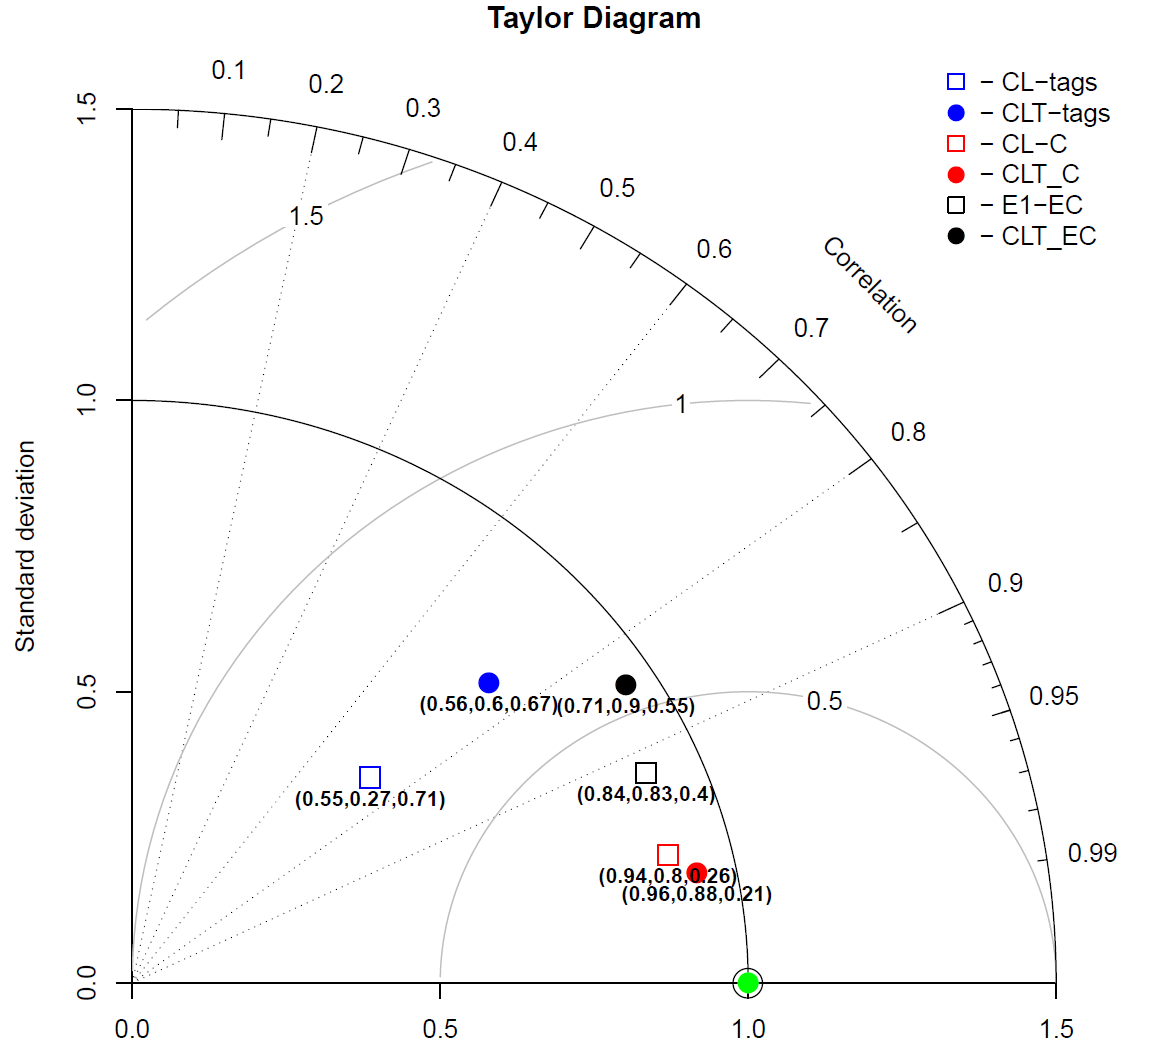
\includegraphics[width=0.95\textwidth]{chapter4/figs/taylor}
		\vspace{0.5cm}
	\caption{Taylor diagram providing three aggregated validation metrics of model fit to the 
data: 1) correlation shown in angular coordinates, 2) standard deviation ratio $\frac{\sigma_{pred}}{\sigma_{obs}}$, shown as a distance from (0,0) point, that is depicted on both, horizontal and vertical axes, and 3) the normalized mean squared error shown as a distance from the best score (1,1,0) depicted by concentric circles. Each filled or empty shape on the Taylor diagram corresponds to three metrics corresponding to the fit by a given model (letters before dash) to a given data (letters after dash): CL (same as E1) denotes the MLE model obtained with catch and length frequency data only, CLT - MLE model with catch, length frequency and tag recapture data, C and EC mean that the fit is measured for catch predicted with catch removal and effort-based methods respectively \citep*[From][]{Senina20b}.}
	\label{fig:taylor}
\end{figure}

Note that the independent data are the data that were not used in the likelihood. We can extend the data time series simply by including several years of data left out for validation, and then to compute the validation scores. However, it is often hard to leave enough data to validate a highly-dimensional model. The best validation of the model with spatial dynamics is its application to a large independent set of data both in time and space and in a comparison with the baseline. An example illustrating this method is described in the recent SEAPODYM study \citep{Senina20a}. The MLE solution obtained for the South Pacific albacore population was applied to simulate the dynamics of the Atlantic stock. Taking into account that the model with optimization performs well on the data that were used in the objective function and usually outperforms the model that was specialized on a different set of data, the MLE was also obtained using the Atlantic Ocean fisheries data. The validity of the South Pacific model was then demonstrated by comparing the statistical metrics computed for its predictions for the Atlantic Ocean population with those computed for the predictions of the Atlantic (baseline) MLE model. 



\addcontentsline{toc}{section}{References}

%\reftitle{References}

\begin{thebibliography}{999}
%\bibitem[Author1(year)]{ref-journal}
%Author~1, T. The title of the cited article. {\em Journal Abbreviation} {\bf 2008}, {\em 10}, 142--149.
%% Reference 2
%\bibitem[Author2(year)]{ref-book1}
%Author~2, L. The title of the cited contribution. In {\em The Book Title}; Editor1, F., Editor2, A., Eds.; Publishing House: City, Country, 2007; pp. 32--58.
%% Reference 3
%\bibitem[Author3(year)]{ref-book2}
%Author 1, A.; Author 2, B. \textit{Book Title}, 3rd ed.; Publisher: Publisher Location, Country, 2008; pp. 154--196.
%% Reference 4
%\bibitem[Author4(year)]{ref-unpublish}
%Author 1, A.B.; Author 2, C. Title of Unpublished Work. \textit{Abbreviated Journal Name} stage of publication (under review; accepted; in~press).
%% Reference 5
%\bibitem[Author5(year)]{ref-communication}
%Author 1, A.B. (University, City, State, Country); Author 2, C. (Institute, City, State, Country). Personal communication, 2012.
%% Reference 6
%\bibitem[Author6(year)]{ref-proceeding}
%Author 1, A.B.; Author 2, C.D.; Author 3, E.F. Title of Presentation. In Title of the Collected Work (if available), Proceedings of the Name of the Conference, Location of Conference, Country, Date of Conference; Editor 1, Editor 2, Eds. (if available); Publisher: City, Country, Year (if available); Abstract Number (optional), Pagination (optional).

\bibitem[Autodif User's Manual, 2021]{Autodif} AUTODIF: A C ++ Array Language Extension with Automatic Differentiation For Use in Nonlinear Modeling and Statistics. \url{https://github.com/admb-project/admb/releases/download/admb-12.3/autodif-12.3.pdf} 

\bibitem [Bard, 1974] {Bard} 
Bard, Y. Nonlinear parameter estimation. Academic Press: New York, 1974.

\bibitem [Griewank and Corliss, 1991] {Griewank} 
Griewank, A.,  Corliss, G.F.  Automatic differentiation of algorithms: theory, implementation, and application. SIAM: Philadelphia, 1991.

\bibitem[Hampton and Fournier, 2001]{Hampton-Fournier}Hampton, J., and Fournier, D.A. 2001. A spatially disaggregated, length-based, age-structured population model of yellowfin tuna (Thunnus albacares) in the western and central Pacific Ocean. Mar. Freshw. Res. 52: 937–963. \url{https://doi.org/10.1071/MF01049}.

\bibitem[Fonteneau, 1996] {Fonteneau} 
Fonteneau, A. Interactions between tuna fisheries: a global review with specific examples from the Atlantic Ocean. In Status of Interactions of Pacific Tuna Fisheries in 1995. Proceedings of the Second FAO Expert Consultation on Interactions of Pacific Tuna Fisheries, Shimizu, Japan, 23–31 January 1995; R.S. Shomura, J. Majkowski, and R.F. Harman, Eds.; FAO Fisheries Technical Paper, 1996; No. 365.

%\bibitem [Langley et al., 2005]{MFCL-SKJ} Langley, A., Hampton, J., Ogura, M.  Stock assessment of skipjack tuna in the western and central Pacific Ocean. Western And Central Pacific Fisheries Commission, Scientific Committee,SA WP4). {\bf 2005}, http://wcpfc.org/sc1/pdf/SC1\_SA\_WP\_4.pdf 

\bibitem[Matear, 1995]{Matear} Matear, R. J. 1995. Parameter optimization and analysis of ecosystem models using simulated annealing: a case study at Station P.  {\em Journal of Marine Research.} {\bf 1995}, {\em 53}, 571--607. 

\bibitem[Otter Research Ltd, 1994]{Fournier} 
Otter Research Ltd. Autodif: a C++ array extension with automatic differentiation for use in nonlinear modeling and statistics. Otter Research Ltd: Nanaimo, Canada, 1994.

\bibitem[SPC Year Book, 2016] {Yearbook} Pacific Community (SPC). 2016. Tuna Fisheries Yearbook. Western and Central Pacific Fisheries Commission, Pohnpei, Federated States of Micronesia.

\bibitem[Pianosi et al., 2016]{Pianosi} 
Pianosi, F., Beven, K., Freer, J., Hall, J., Rougier, J., Stephenson, D., and Wagener, T. Sensitivity analysis of environmental models: A systematic review with practical workflow. Environ. {\em Modell. Softw.} {\bf 79}, 214–-232. \url{https://doi.org/10.1016/j.envsoft.2016.02.008}.

%continue formatting from here

\bibitem[Robinson and Lermusiaux, 2002]{Robinson} Robinson, A.R., Lermusiaux, P. F. J. 2002. Data assimilation for modeling and predicting coupled physical biological interactions in the sea. From \textit {The Sea}, Volume 12, edited by Allan R. Robinson, James J. McCarthy, and Brian J. Rothschild. John Wiley \& Sons, Inc., New York. 475-536.

\bibitem[Saltelli et al., 2008]{Saltelli} Saltelli, A., Ratto, M., Andres, T., Campolongo, F., Cariboni, J., Gatelli, D., et al. 2008. Global sensitivity analysis. The Primer. John Wiley and Sons.

\bibitem[Senina et al., 2008]{Senina08} Senina, I., Sibert, J., and Lehodey, P. 2008. Parameter estimation for basin-scale ecosystem-linked population models of large pelagic predators: Application to skipjack tuna. Prog. Oceanogr. 78: 319–335. doi:10.1016/j.pocean.2008.06.003.

%\bibitem[Senina et al., 2012]{Senina12} Senina, I., Royer, F., Lehodey, P., Hampton, J., Nicol, S., Ogura, M., et al. 2012. Integrating conventional and electronic tagging data into SEAPODYM. Pelagic Fish. Res. Prog. Univ. Hawaii Manoa Newslett. 16(1): 9–14.

\bibitem[Senina et al., 2020a]{Senina20a} Senina, I., Lehodey, P., Hampton, J. and J. Sibert. 2020a. Quantitative modelling of the spatial dynamics of South Pacific and Atlantic albacore tuna populations. \textit{Deep Sea Res. II}  175,  doi.org/10.1016/j.dsr2.2019.104667).  

\bibitem[Senina et al., 2020b]{Senina20b} Senina, I., Lehodey, P., Sibert, J. and J. Hampton. 2020b. Integrating tagging and fisheries data into a spatial population dynamics model to improve its predictive skills. \textit{Can. J. Aquat. Fish. Sci.} 77, 576–593.

\bibitem[Senina et al., 2020c]{Senina2020c} Senina, I., Lehodey, P., Nicol, S., Scutt Phillips, J., Hampton, J., 2020c. SEAPODYM: revisiting bigeye reference model with conventional tagging data. WCPFC-SC16-2020.

\bibitem[Sibert et al., 1999]{Sibert} Sibert, J.R., Hampton, J., Fournier, D.A., Bills, P.J. 1999. An advection-diffusion-reaction model for the estimation of fish movement parameters from tagging data, with application to skipjack tuna ({\it Katsuwonus pelamis}). \textit {Can. J. Fish. Aquat. Sci.} 56, 925-938. 

%\bibitem[Sibert and Hampton, 2003]{Sibert-Hampton} Sibert, J., Hampton, J. 2003. Mobility of tropical tunas and the implications for fishery management. \textit {Marine Policy} 27: 87-95.
%Procedings of the Second FAO Expert Consultation on Interactions of Pacific Ocean Tuna Fisheries, Shimizu, Japan, 23-31 January, 1995; FAO Fish. Tech. Pap. 365:402-418, Rome, 1996, 612pp. edited by R. S. Shomura, J. Majkowski, and R. F. Harman. 1996.

\bibitem[Taylor, 2001]{Taylor} Taylor, K.E. 2001. Summarizing multiple aspects of model performance in a single diagram. J. Geophys. Res. 106: 7183–7192. \url{https://doi.org/10.1029/2000JD900719}.

\bibitem[Vallino, 2000]{Vallino} Vallino, J.J. 2000. Improving marine ecisystem models: use of data assimilation and mesocosm experiments. \textit {Journal of Marine Research.} 58, 117-164.

\bibitem[Worley, 1991]{Worley} Worley, B. 1991. Experience with the forward and reverse mode of GRESS in contaminent transport modeling and other applications. In Griewank, A. and G.F. Corliss. Automatic differentiation of algorithms: theory, practice and application. SIAM, Philadelphia.

\end{thebibliography}

%%%%%%%%%%%%%%%%%%%%%%%%%%%%%%%%%%%%%%%%%%%%%%%%%%%%%%%%%%%%%%%%%%%%%%%%%%%%%%%%%%%%%%%%%%%%%%%%%%%

%%% Local Variables:
%%% TeX-master: "../Seapodym_user_manual.tex"
%%% End: